% ****** Start of file apssamp.tex ******
%
%   This file is part of the APS files in the REVTeX 4 distribution.
%   Version 4.0 of REVTeX, August 2001
%
%   Copyright (c) 2001 The American Physical Society.
%
%   See the REVTeX 4 README file for restrictions and more information.
%
% TeX'ing this file requires that you have AMS-LaTeX 2.0 installed
% as well as the rest of the prerequisites for REVTeX 4.0
%
% See the REVTeX 4 README file
% It also requires running BibTeX. The commands are as follows:
%
%  1)  latex apssamp.tex
%  2)  bibtex apssamp
%  3)  latex apssamp.tex
%  4)  latex apssamp.tex
%
\documentclass[prb,aps,twocolumn,preprintnumbers,amsmath,amssymb]{revtex4}
%\documentclass[preprint,showpacs,preprintnumbers,amsmath,amssymb]{revtex4}

% Some other (several out of many) possibilities
%\documentclass[preprint,aps]{revtex4}
%\documentclass[preprint,aps,draft]{revtex4}
%\documentclass[prb,twocolumn,showpacs,preprintnumbers,amsmath,amssymb]{revtex4}% Physical Review B

\usepackage{graphicx}% Include figure files
\usepackage{dcolumn}% Align table columns on decimal point
\usepackage{bm}% bold math
\usepackage[utf8]{inputenc}
\usepackage[spanish,es-tabla]{babel}
\usepackage{url}
\newcolumntype{P}[1]{>{\centering\arraybackslash}p{#1}}
\newcolumntype{M}[1]{>{\centering\arraybackslash}m{#1}}


\begin{document}

\title{Radioactividad}% Force line breaks with \\

\author{Alejandro Hernández A.}%
 \email{a.hernandez105@uniandes.edu.co}
\author{Daniel Sánchez M.}%
 \email{d.sanchez462@uniandes.edu.co}
\affiliation{%
Departamento de Física\\ Universidad de los Andes, Bogotá, Colombia.\\
}%

\date{1 de octubre de 2015}% It is always \today, today,
             %  but any date may be explicitly specified

\begin{abstract}
Este informe presenta los datos obtenidos al medir la radioactividad de diversas fuentes previamente proporcionadas con la ayuda de un contador de Geiger. Dado a que se realizaron multiples experimentos, el único dato que vale le pena mostrar aquí es la radiación natural por minuto, para la cual se obtuvo un resultado de $r_{natural} = 25.6 \pm 1$ con unidades del contador de Geiger. Los demás resultados y todos los comentarios de los mismos se muestran en la sección de \textbf{RESULTADOS Y ANÁLISIS}.\\

\noindent \textbf{Conceptos clave:} Radiación, tipos de radiación, fuentes de radiación, radio, contador de Geiger-Müller.
\end{abstract}
                             
\maketitle

\section{INTRODUCCIÓN}
En el año de 1986 Henri Becquerel observó que rayos emitidos desde ciertos materiales podían atravesar el papel negro además de causar el empañamiento de una placa fotografica no expuesta. Su estudiante doctoral Marie Curie descubrió que solo ciertos elementos quimicos podían producir estos rayos de energía. Precisamente fue Marie Curie quien nombró a este comportamiento como radioactividad \cite{wikipedia}. \\

La radioactividad es un fenómeno mediante el cual se transmite energía en forma de ondas o partículas a través del vacío o de un material. Existen diferentes tipos de radiación en la naturaleza, entre ellas, la radiación electromagnética, que incluye ondas de radio, luz visible y rayos x; y la 	radiación de partículas, como la radiación $\alpha$, $\beta$ y la radiación de neutrones \cite{wikipedia}.\\

Allende de lo mencionado anteriormente, la radiación es típicamente clasificada como ionizante o no-ionizante dependiendo de la energía de las partículas emitidas. La radiación ionizante tiene energías del orden de los $10\ eV$, la cual es suficiente para ionizar átomos y moléculas, además de romper enlaces químicos, de ahí el carácter ionizante de la misma. Este fue el tipo de radiación usada en el laboratorio y el pricipal motivo para ello es que dicho tipo de radiactividad puede ser medidad mediante un contador de Geiger-Müller.\\

La radiación ionizante, como se mencionó previamente, se caracteriza principalmente por ser capaz de remover electrones de sus átomos o de moléculas. Está compuesta por partículas masivas y núcleos atómicos viajando a velocidades relativistas, además de ondas electromagnéticas de altos niveles de energía. Una gran parte de la radiación ionizante conocida proviene del decaimiento de elementos radioactivos, ya que la energía necesaria para que este decaimiento ocurra es significativamente mayor a la necesaria para ionizar cualquier tipo de átomo. Otras partículas ionizantes como muones, mesones, positrones y neutrones, provienen de la interacción de rayos cósmicos con la atmósfera del planeta, produciendo una radiación de fondo de baja intensidad presente en cualquier lugar de la superficie terrestre.\\

Algunas particularidades de los tres tipos de radiación más comunes se mencionan a continuación. 

\subsection{Radiación Gamma}
Los rayos gamma son un tipo de radiación electromagnética (fotones) producida generalmente por elementos radiactivos o por procesos subatómicos como la aniquilación de un par positrón-electrón. Debido a las altas energías que poseen, los rayos gamma constituyen un tipo de radiación ionizante capaz de penetrar en la materia más profundamente que la radiación alfa y la beta (que serán explicadas posteriormente). Pueden causar grave daño al núcleo de las células, razón por la cual se usan para esterilizar equipos médicos y alimentos\cite{hyperphyisics}. 


\subsection{Radiación Alfa}

La radiación alfa se compone de núcleos de helio (dos protones y dos neutrones) viajando a velocidades relativistas. Dichos núcleos se generan en reacciones nucleares o desintegración radiactiva de otros núclidos que se transmutan en elementos más ligeros mediante la emisión de dichas partículas. Su capacidad de penetración es pequeña; en la atmósfera pierden rápidamente su energía cinética, porque interactúan fuertemente con otras moléculas debido a su gran masa y carga eléctrica, creando una cantidad considerable de iones por centímetro de longitud recorrida. En general no pueden atravesar espesores de varias hojas de papel \cite{hyperphyisics}.\\

En el laboratorio se verificó que la radiación alfa no puede atravesar muchas hojas de papel y esta propiedad puede ser usada para caracterizar el tipo de radiación emitida por diversas fuentes. 


\subsection{Radiación Beta}

La radiación beta es  un tipo de forma de radiación ionizante que se compone de electrones o positrones con alta energía que son emitidos por cierto tipo de núcleos radioactivos tales como el Potasio 40. Estas partículas pueden atravesar ciertos materiales que bloquean la radiacióm alfa, lo cual permite nuevamente caracterizar ciertos materiales \cite{hyperphyisics}.

\section{Montaje Experimental}

En general el montaje consiste de un contador de Geiger-Müller, diversas bases para sostener los elementos usados y una muestra radioactiva, tal como se ilustra en la figura \ref{fig: montaje}.

\begin{figure}[h!]
	\centering
	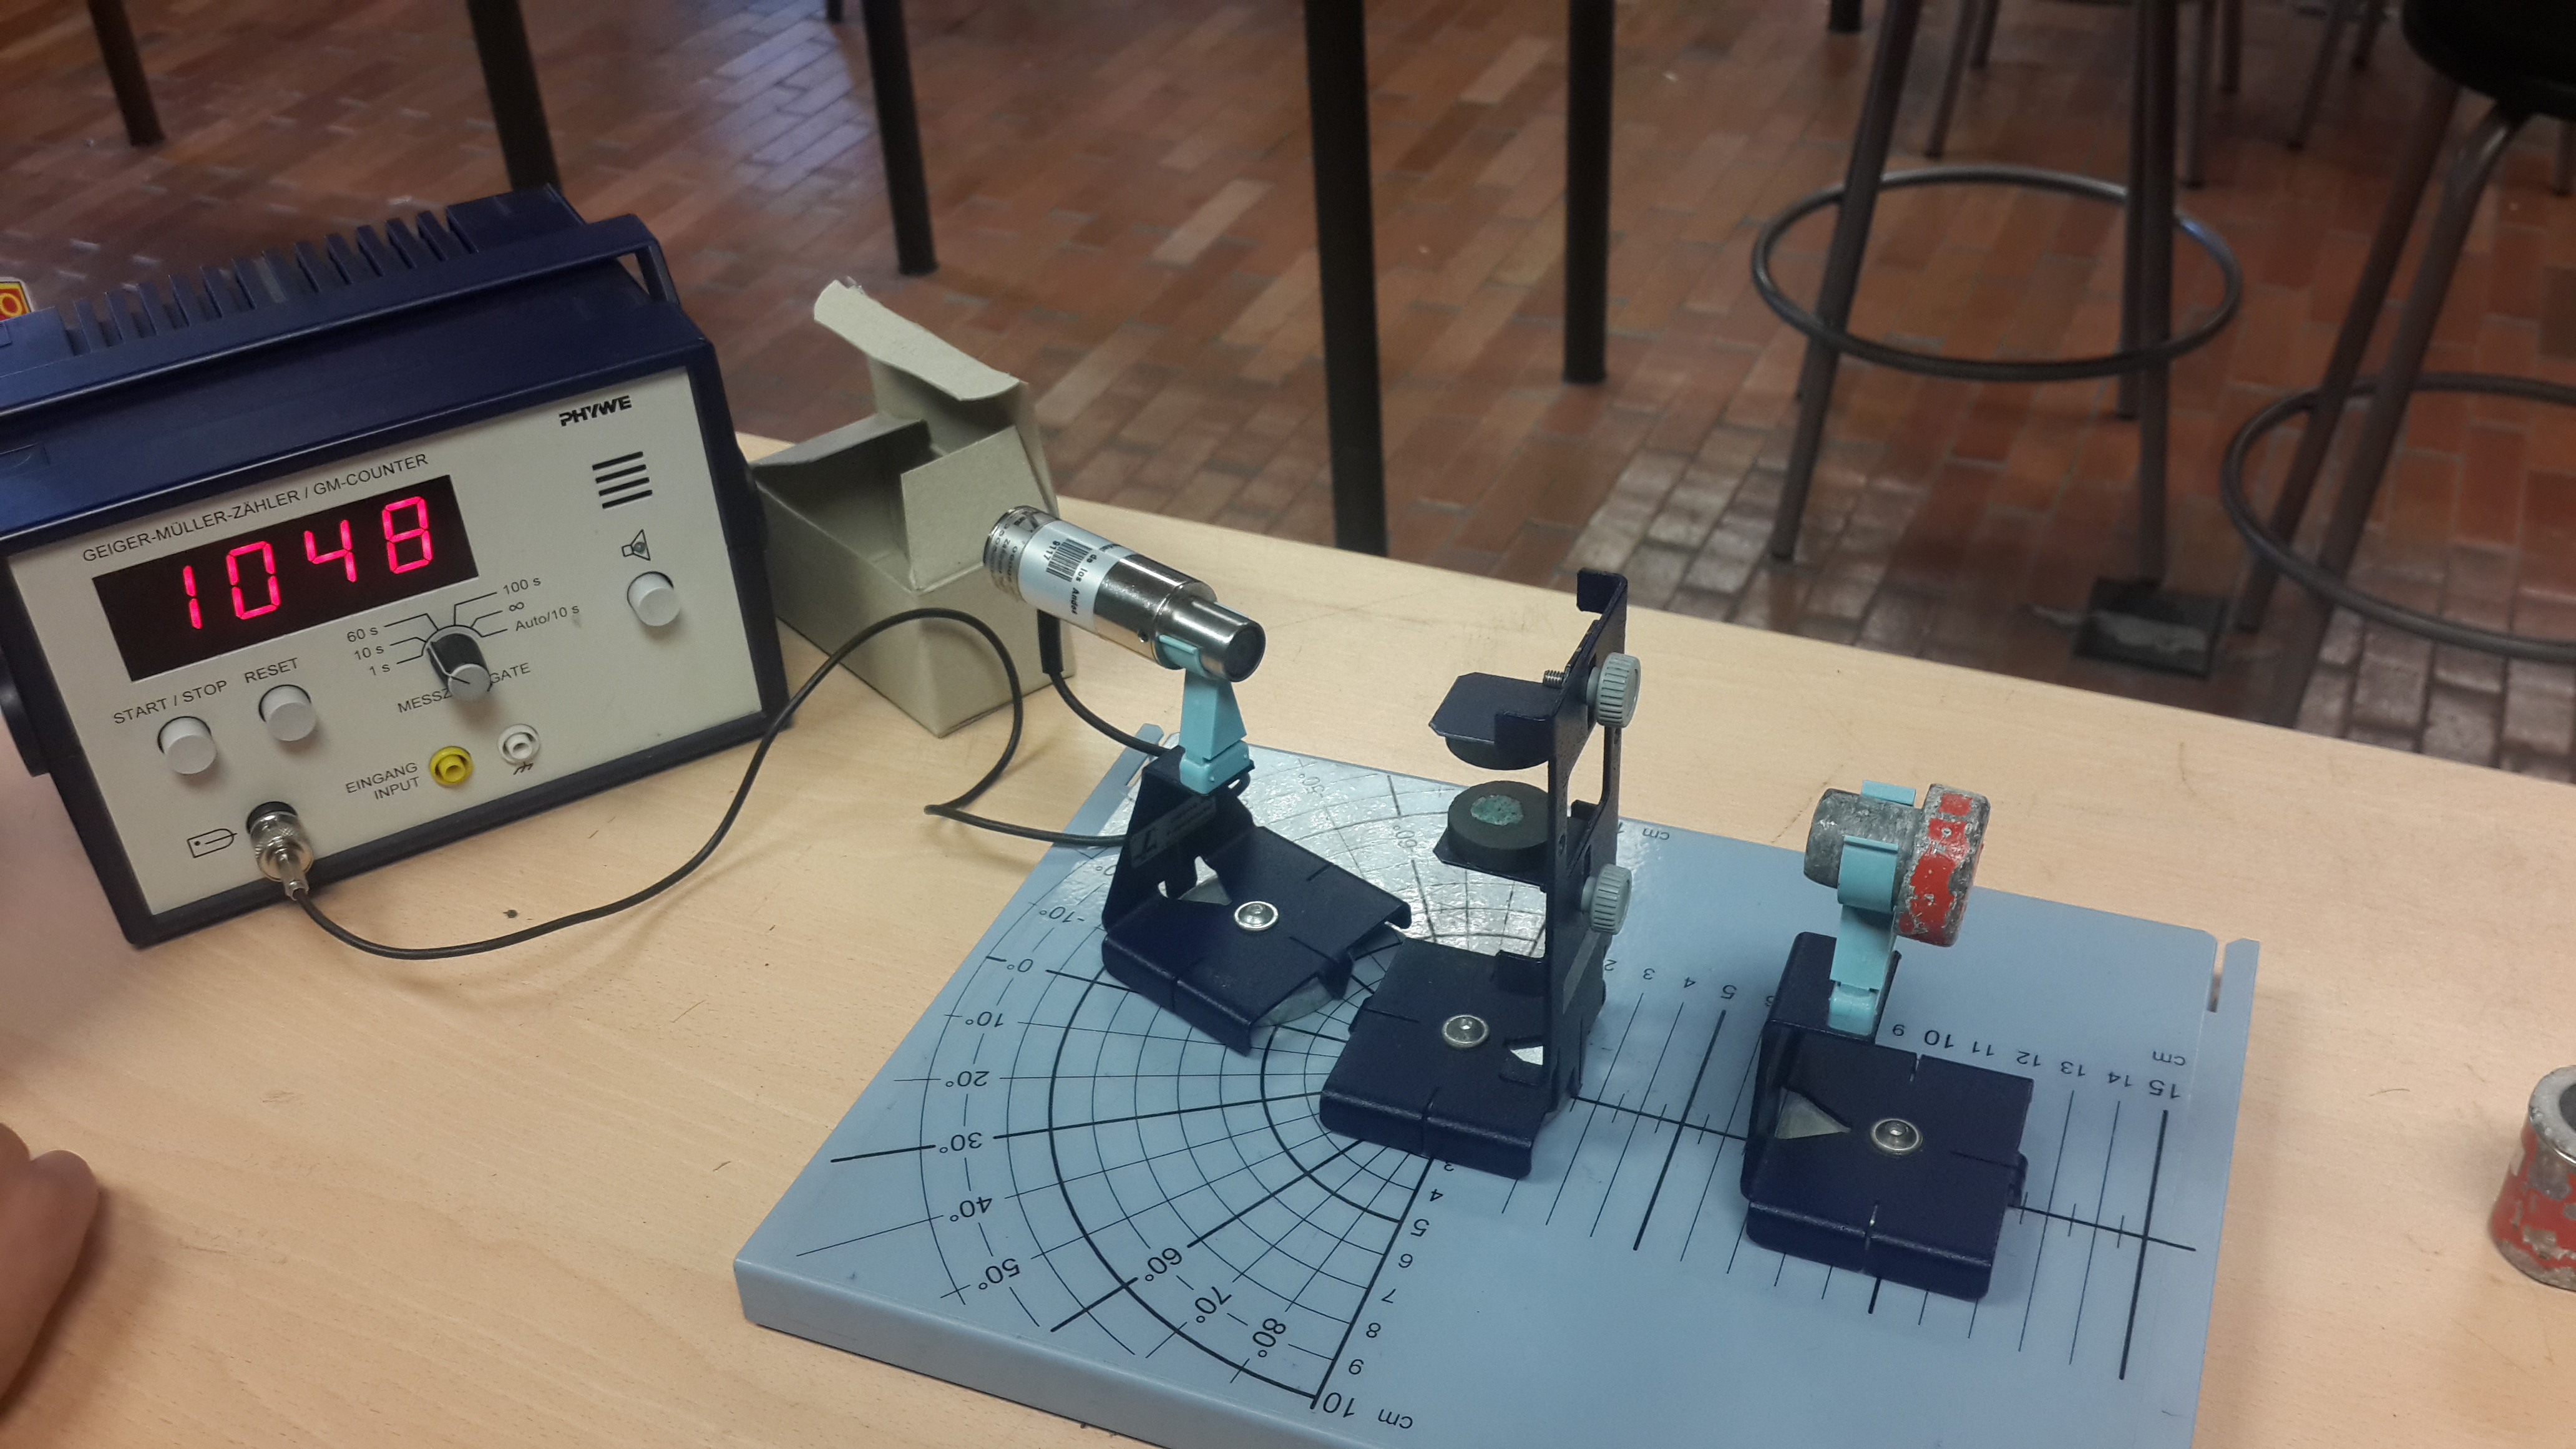
\includegraphics[width=0.5\textwidth]{montaje}
	\caption{ Montaje experimental usado en la práctica. }
	\label{fig: montaje}
\end{figure}

Usualmente la radiación natural o artificial, ionizante o no, está fuera del espectro visible, excepto cuando se tienen fenómenos como \textit{Cherenkov Radiation} \footnote{La radiación Cherenkov es producida cuando una partícula cargada como un electrón pasa a través de un dieléctrico con una velocidad más grande que la velocidad de propagación de la luz en dicho medio.\\} o \textit{Radioluminiscencia}. Por tal motivo es necesario un instrumento capaz de detectar la radiación emitida por una determinada muestra. Precisamente esa es la función del contador Geiger-Müller, que fue el dipositivo fundamental durante la práctica.\\

El contador de Geiger está formado por un tubo con un fino hilo metálico a lo largo de su centro. El espacio entre ellos (entre el hilo y el tubo), está aislado y relleno de un gas inerte, tal como se ilustra\footnote{Imagen  obtenida de http://kaffee.50webs.com/Science/labs\\/Chem/Lab-Geiger.Counter.html\\} en la figura \ref{fig: contador}.\\

\begin{figure}[h!]
	\centering
	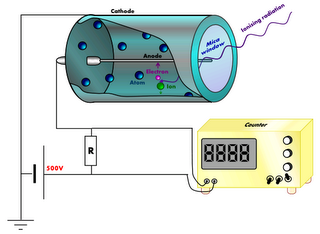
\includegraphics[width=0.5\textwidth]{geiger}
	\caption{ Contador de Geiger. }
	\label{fig: contador}
\end{figure}

Un ión o electrón que penetra en el tubo desprende electrones de los átomos del gas. Debido a la diferencia de potencial del hilo central con la superficie que recubre el contador, estos electrones son atraídos hacia el hilo, aumentando su energía. Dichos electrones colisionan con los átomos y liberan más electrones, hasta que el proceso se convierte en una avalancha que produce un pulso de corriente detectable. Relleno de un gas adecuado, el flujo de electricidad se detiene por sí mismo o incluso el circuito eléctrico puede ayudar a detenerlo.
Al instrumento se le llama un contador debido a que cada partícula que pasa por él produce un pulso idéntico, permitiendo contar las partículas pero sin tener información sobre su identidad o su energía.


\section{Resultados y análisis}

\subsection{Radiación de fondo}
En este experimento se midió la radiación de fondo del salón de clase. No se colocaron frente al medidor muestras de ningún tipo, y se dejo efectuar el conteo de la radiación natural del ambiente. Los datos se muestran en la tabla \ref{tabla1}.

\begin{table}[h!]
	\caption{\label{tabla1}Conteos para la radiación natural.}
	\begin{ruledtabular}
		\begin{tabular}{|M{3.5cm}|M{4.5cm}|}
			Número de la medición & $\frac{C_{0}}{conteos / 60\ s}$\\
			\hline
			1 & 19 \\
			2 & 14 \\
			3 & 19 \\
			4 & 22 \\
			5 & 16 \\
		\end{tabular}
	\end{ruledtabular}
\end{table}

El promedio fue de 18 conteos/min. con error \cite{error} de 9 conteos/min, los cuales van a ser considerados para los cálculos sobre mediciones posteriores de muestras radioactivas. \\

Teniendo en cuenta que no se tenían muestras radioactivas cerca del contador, se pudo verificar que existe radiacion en el ambiente cotidiano, por lo cual se concluye que dicho fenómeno natural es algo con lo que los seres vivos interactuamos constantemente.\\

Podemos concluir además que:

\begin{itemize}
	\item No se tienen un conteo constante en las mediciones puesto que existe una desviación estándar de los datos de 3,08, evidenciando una alta dispersión de los mismos. 
	
	\item La radiación medida puede venir de múltiples fuentes naturales, pero posiblemente se compone en su mayoría de radiación cósmica. Los materiales de construcción, el suelo y el agua contienen también pequeñas concentraciones de materiales radioactivos pero su intensidad es muy baja para ser medida por el contador. 
\end{itemize}

\subsection{Variaciones aleatorias en los conteos}

En este experimento se realizaron 50 mediciones de 10 segundos cada una, en las cuales se ponía de forma vertical el tubo contador, apuntando directamente hacia una manta radioactiva tal y como se muestra en la figura \ref{fig: manta}.

\begin{figure}[h!]
	\centering
	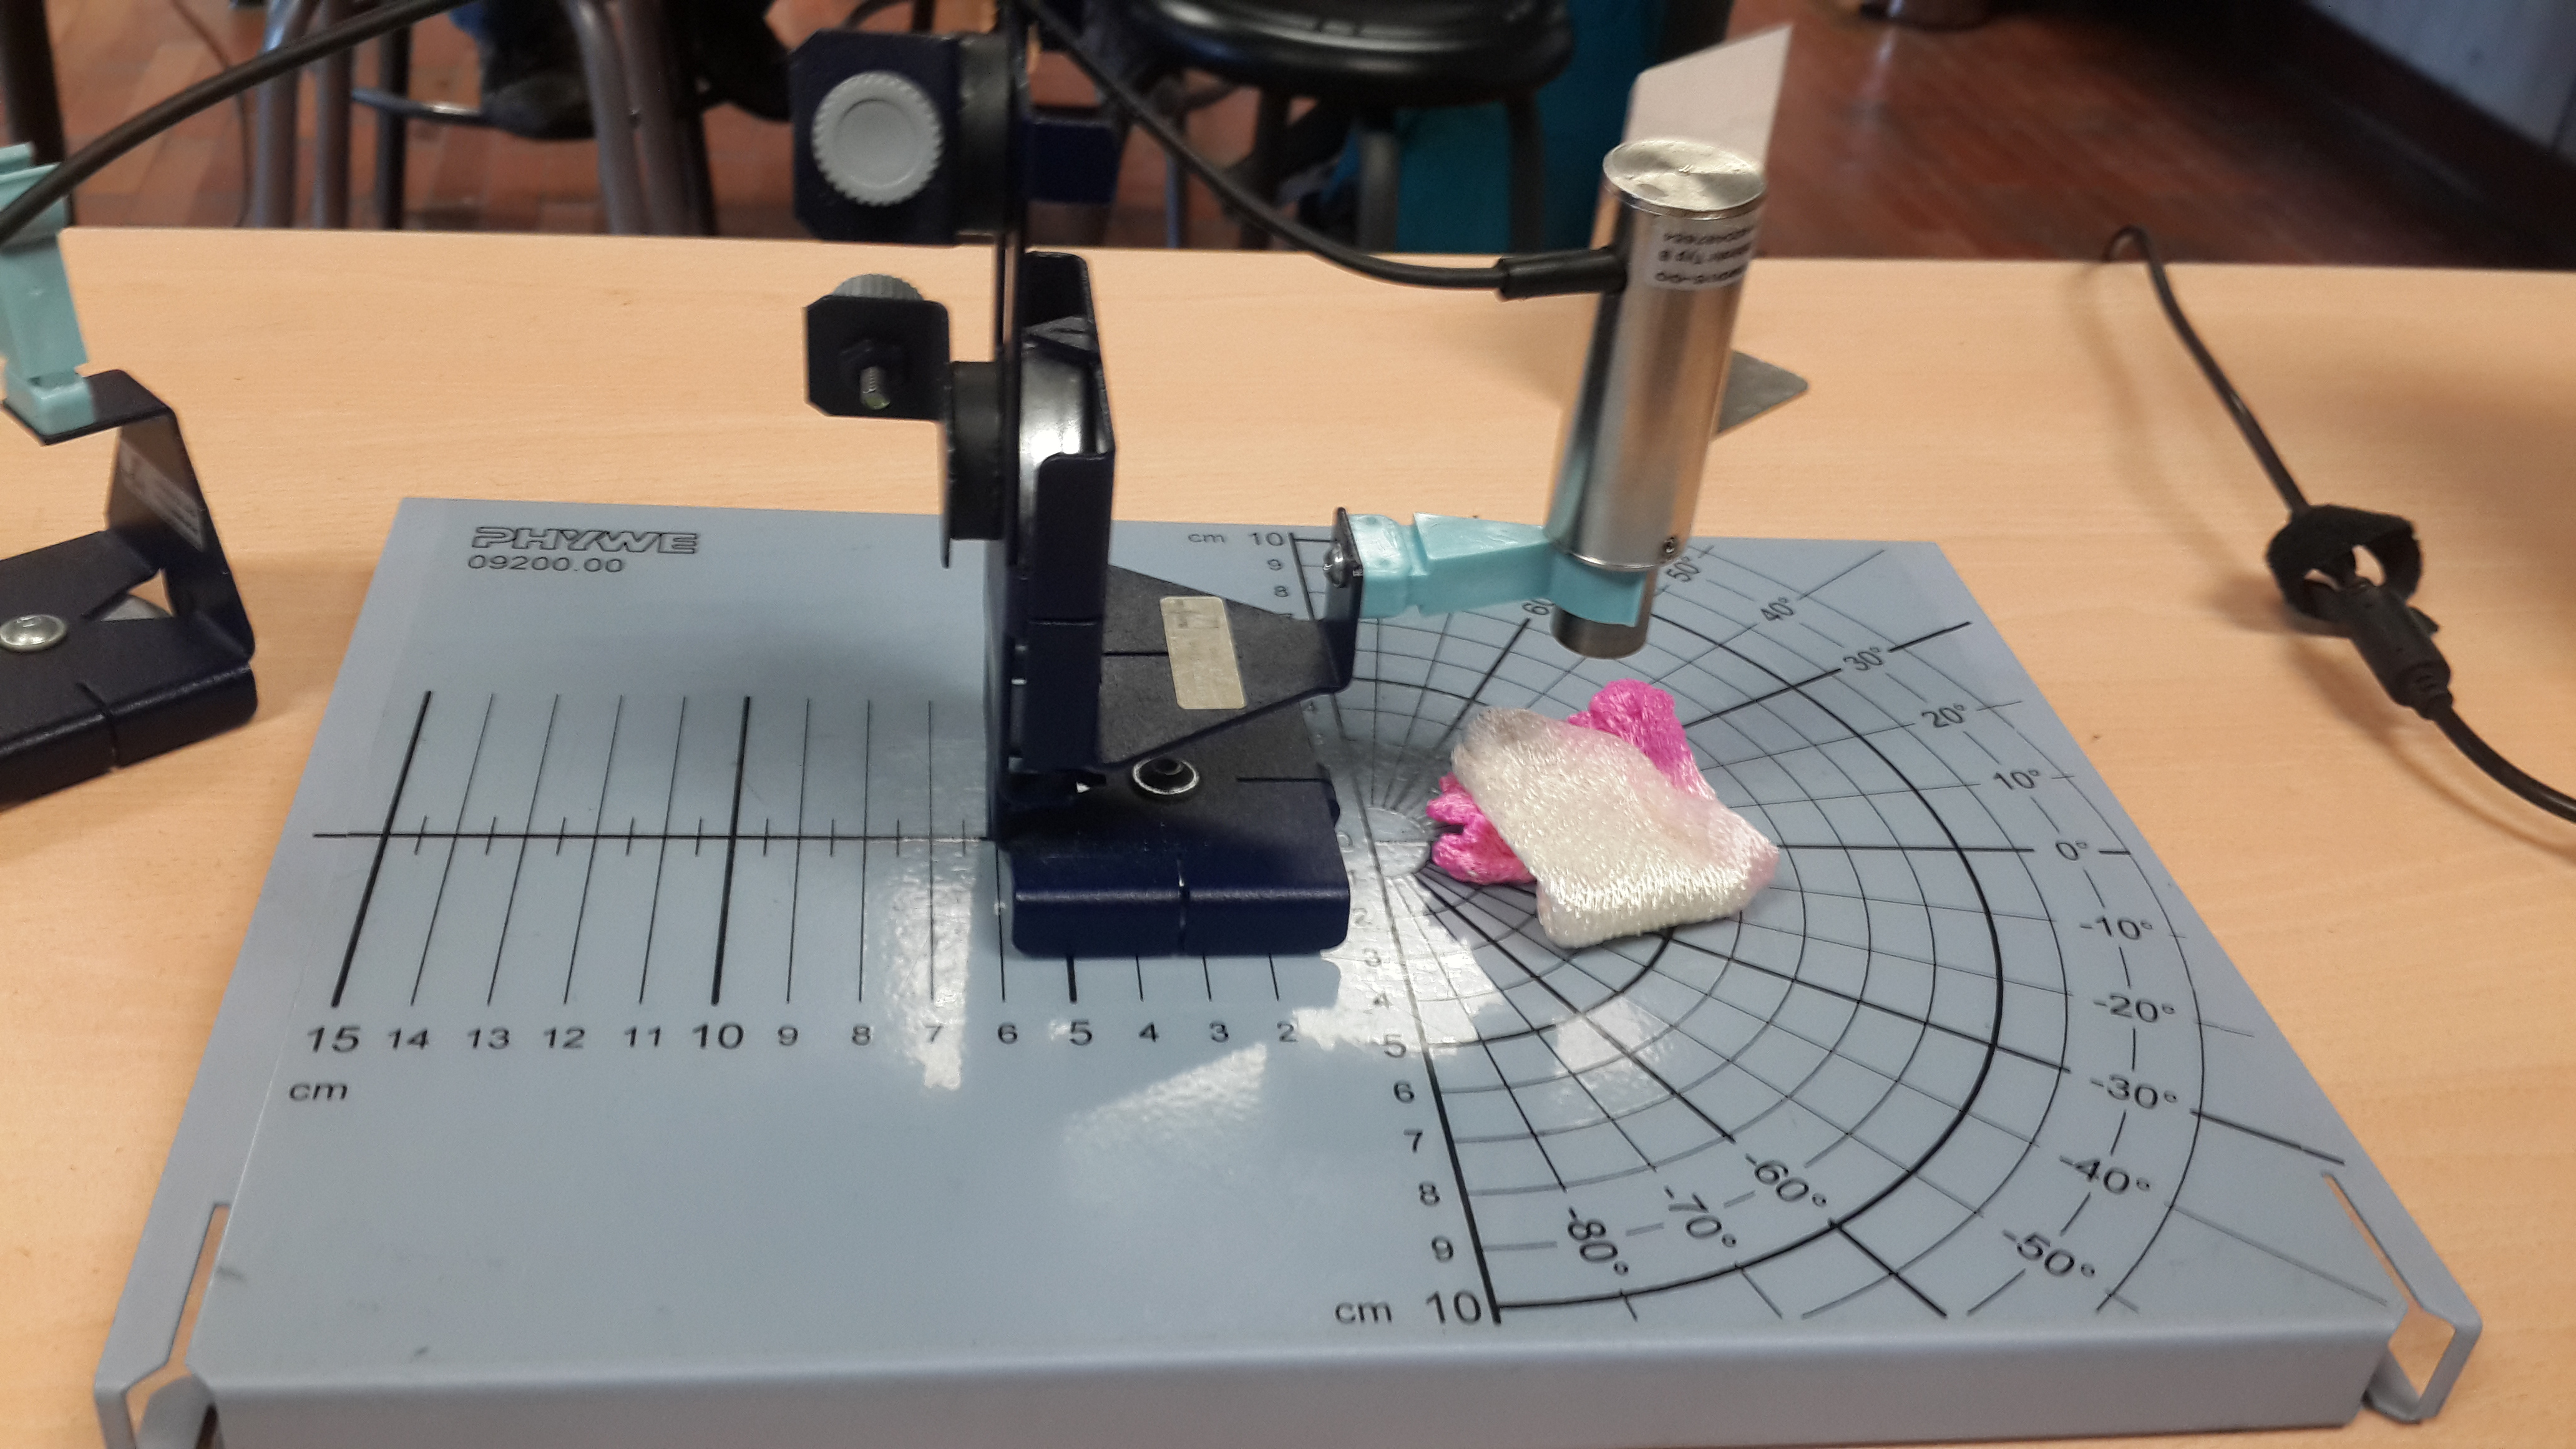
\includegraphics[width=0.5\textwidth]{manta}
	\caption{ Toma de datos de los niveles de radiacion de una manta. }
	\label{fig: manta}
\end{figure}

Los datos obtenidos se muestran en la tabla \ref{tabla2}.\\

\begin{table}[h!]
	\caption{\label{tabla2}Conteos para las variaciones de la radiación natural.}
	\begin{ruledtabular}
		\begin{tabular}{|M{1.cm}|M{1.cm}|M{1.cm}|M{1.cm}|M{1.cm}|M{1.cm}|}
			Med. \# & Cont.  10 s & Med. \# & Cont.  10 s & Med. \# & Cont.  10 s\\
			\hline
			1 & 101 & 18 & 79 & 35 & 86\\
			2 & 72 & 19 & 76 & 36 & 92\\
			3 & 80 & 20 & 95 & 37 & 77\\
			4 & 96 & 21 & 105 & 38 & 87\\
			5 & 70 & 22 & 68 & 39 & 82\\
			6 & 84 & 23 & 114 & 40 & 101\\
			7 & 91 & 24 & 102 & 41 & 91\\
			8 & 89 & 25 & 87 & 42 & 86\\
			9 & 76 & 26 & 88 & 43 & 69\\
			10 & 86 & 27 & 93 & 44 & 80\\
			11 & 79 & 28 & 79 & 45 & 86\\
			12 & 96 & 29 & 92 & 46 & 85\\
			13 & 105 & 30 & 76 & 47 & 97\\
			14 & 88 & 31 & 85 & 48 & 93\\
			15 & 79 & 32 & 101 & 49 & 92\\
			16 & 80 & 33 & 93 & 50 & 87\\
			17 & 79 & 34 & 77 &  & \\
		\end{tabular}
	\end{ruledtabular}
\end{table}

El promedio de estas mediciones fue $\bar{C} = 87.04$ conteos/10 s con un error de $9.32$ conteos/10 s. Dado lo anterior, se obtuvo un error porcentual de $10.72 \%$ en estas mediciones, lo cual es aceptable teniendo en cuenta las múltiples fuentes de error, entre ellas la ralización de otros experimentos de radiación con fuentes como el radio el mesas aledañas y el hecho de que al pricipio no sabíamos a qué parte de la manta apuntar con el contador, lo cual rodujo medidas incoherentes al principio del experimento.\\

Las medidas que más difieren del valor promedio fueron la medición \# 2 y la medición \# 23, registrando valores de $72$ y $114$ conteos respectivamente, los cuales están claramente fuera del error de la medida, potencialmente por las fuentes de error explicadas previamente.\\

La gráfica de frecuencias solicitada se muestra en la figura \ref{fig: frecuencia}.

\begin{figure}[h!]
	\centering
	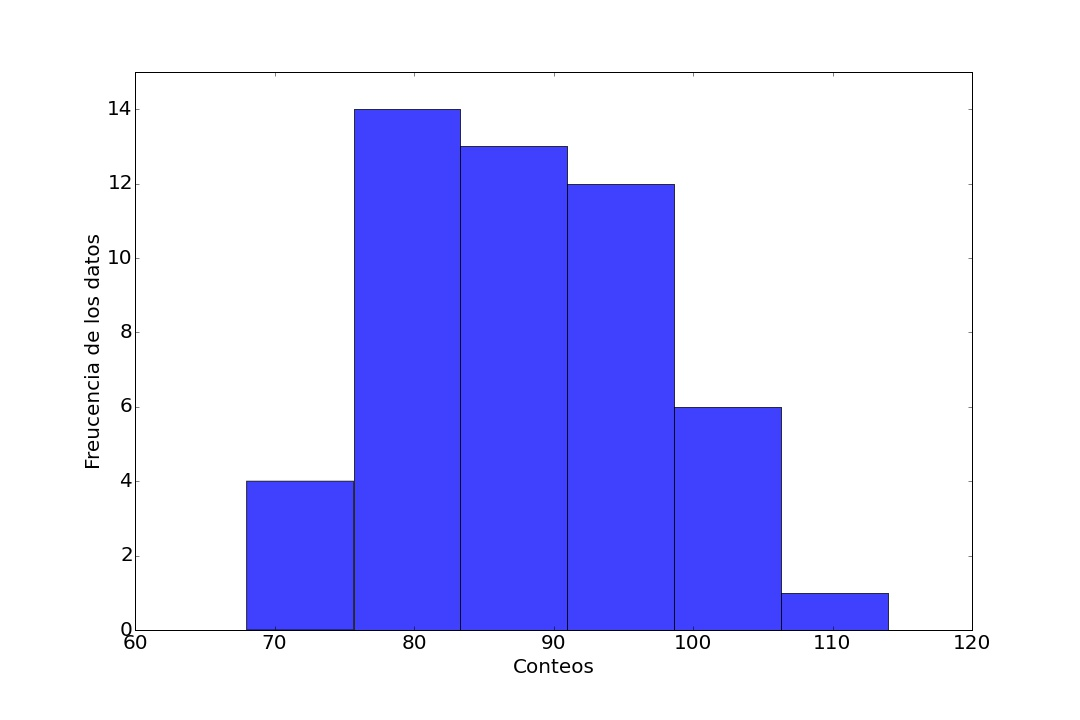
\includegraphics[width=0.5\textwidth]{frequency}
	\caption{ Gráfica de la frecuencia de datos de los niveles de radiacion de un manta. }
	\label{fig: frecuencia}
\end{figure}

Dicha gráfica evidencia claramente la concentración de los datos alrededor del promedio calculado previamente y ademas perimite concluir que los datos extremos de las mediciones \# 2 y \# 23 son casos aislados con frecuencia baja. Además de lo anterior, calculamos que el $70 \ \%$ de los datos están dentro del error calculado para la medida $87.04 \pm 9.32$. Este valor indica que se realiza una buena toma de datos dado que el valor teórico esperado de los datos dentro de ese rango es del $68.3\ \%$.

\subsection{Rocas radioactivas}
 
Al igual que en el experimento anterior, el montaje experimental se muestra en la figura \ref{fig: montaje}. En este caso, el objetivo es determinar a partir de los conteos hechos con el contador Geiger-Müller si una sustancia es radioactiva o no, es decir, si produce la suficiente radiación ionizante. Se tomaron 3 muestras de columbita (mineral proporcionado dentro de los elementos de laboratorio) y medimos los conteos detectados. En la tabla \ref{tabla3} se pueden observar los resultados de estas mediciones.

\begin{table}[h!]
	\caption{\label{tabla3}Conteos para diversas muestras de columbita.}
	\begin{ruledtabular}
		\begin{tabular}{|M{1.cm}|M{1.cm}|M{1.cm}|M{1.cm}|M{1.cm}|M{1.cm}|}
			Sust. & $C_{1}$ / 60 s & $C_{2}$ / 60 s & $C_{3}$ / 60 s & $C_{4}$ / 60 s & $\bar{C}$ /\ \ \ \  60 s\\
			\hline
			Aire & 19 & 21 & 19 & 13 & 18\\
			Colum. 1 & 33 & 40 & 34 & 40 & 36.75\\
			Colum. 4 & 47 & 49 & 35 & 39 & 42.5\\
			Colum. 7 & 103 & 79 & 117 & 89 & 97\\
		\end{tabular}
	\end{ruledtabular}
\end{table}

A partir de los datos mostrados en la tabla anterior se evidencia claramente un mayor conteo para la columbita 7 que para las demás. A partir de lo consultado en REFERENCIA se espera que para una sustancia radiactiva se obtengan al rededor de 200 conteos/min., razón por la cual podemos concluir que ninguna de las muestras analizadas podrían ser consideradas radioactivas, y a pesar de que la columbita 7 es que más actividad resgistró de todas, con un conteo promedio de $\bar{C} = 79$ al tener en cuenta al aire, este conteo no es lo suficiente alto para considerar dicho mineral como una amenaza para la salud. \\

Además de lo anterior, podemos concluir que el contador de Geiger es un instrumento extremadamente útil para la detección de materiales radioactivos.

\subsection{Sales radioactivas}
 
Nuevamente se usó el mismo montaje de los experimentos anteriores. En este experimento se analizaron los conteos obtenidos cuando ponemos diferentes tipos de sales bajo el tubo contador. Los resultados obtenidos y las sales usadas se muestran en la tabla \ref{tabla4}.

\begin{table}[h!]
	\caption{\label{tabla4}Conteos para diversas muestras de sales.}
	\begin{ruledtabular}
		\begin{tabular}{|M{1.4cm}|M{1.4cm}|M{1.4cm}|M{1.4cm}|M{1.4cm}|}
			Sust. & $C_{1}$/\ \ \ \ \ \ \ \ \ 100 s & $C_{2}$/\ \ \ \ \ \ \ \ \ 100 s & $C_{3	}$/\ \ \ \ \ \ \ \ \ 100 s & $\bar{C}$/\ \ \ \ \ \ \ \ \ 100 s\\
			\hline
			Aire & 35 & 30 & 36 & 33.66 \\
			$KCL$ & 40 & 50 & 43 & 44.33 \\
			$CaCl_{2}$ & 33 & 32 & 24 & 29.66\\
			$CuSO_{4}$ & 28 & 31 & 20 & 26.33\\
		\end{tabular}
	\end{ruledtabular}
\end{table}

Es importante resaltar que la radiación del aire aumentó ligeramente para estas emmisiones y la razón para esto es que en la mesas contiguas estaban trabajando con muestras de radio al momento de realizar las mediciones. A pesar de lo mencionado anteriormente, ninguna de estas sales puede ser considerada como radioactiva de acuerdo al conteo de corte previamente aludido. La sal que menos radiación emitió fue el sulfato de cobre y la que más emitió fue la sal de cocina, algo realmente o esperado dado que se esperaba que la sal de cocina fuera la de menor emisión puesto que es una sustancia para el consumo humano. Dado esto, se puede concluir que las sales examinadas no representan ningún peligro para la salud humana.\\

Ahora bien, note que al tener en cuenta al aire para calcular los promedios de conteos  se obtienen valores negativos tanto para el cloruro de calcio como para el sulfato de cobre. Este valor negativo puede explicarse teniendo en cuenta el trabajo de grupos aledaños con muestras altamente radioactivas como el radio, además de que dado que el tubo contador se ubica lo suficientemente cerca de la muestra, es muy probable que dicho instrumento solo haya detectado la radiación de la  muestra y no la radiación del aire. Por tanto, en todas los experimentos de este tipo, en los que el contador se encuentre de forma vertical sobre la muestra y a una distancia tan corta, y sobre todo cuando trabajamos con bajos conteos como en este caso, es posible que se deba ignorar la radiación del aire y tratar de no realizar mediciones mientras otros grupos trabajen con muestras altamente radioactivas como el radio.

\subsection{Distinción entre los tipos de radiación}

El objetivo de los experimentos eplicados a continuación era determinar el tipo y la intensidad de la radiación producida por rocas radioactivas (columbita) y por una manta incandescente.\\

En el primer experimento se utilizó la columbita 7 y se evaluó como variaban sus conteos dependiendo del material que se imponía entre el contador y la columbita. Dado a una observación sobre el hehcho de que había un lado de la columbita que emitía más radiación, primero se determino el lado que más emitía con el fin de poder evaluar correctamente la parte del bloqueo. Los resultados de este experimento se muestran en la tabla \ref{tabla5}.

\begin{table}[h!]
	\caption{\label{tabla5}Conteos para la columbita 7 teniendo en cuenta materiales de bloqueo.}
	\begin{ruledtabular}
		\begin{tabular}{|M{1.4cm}|M{1.4cm}|M{1.4cm}|M{1.4cm}|M{1.4cm}|}
			Sust. & $C_{1}$/\ \ \ \ \ \ \ \ \ 100 s & $C_{2}$/\ \ \ \ \ \ \ \ \ 100 s & $C_{3}$/\ \ \ \ \ \ \ \ \ 100 s & $\bar{C}$/\ \ \ \ \ \ \ \ \ 100 s\\
			\hline
			Lado 1 & 160 & 167 & 159 & 162 \\\hline
			Lado 2 & 199 & 247 & 262 & 236 \\\hline
			Lado 2 - Papel & 219 & 209 & 201 & 209.66\\\hline
			Lado 2 - Placa de plomo & 51 & 55 & 51 & 52.33\\
		\end{tabular}
	\end{ruledtabular}
\end{table}

Dado que se encontró que el lado que más emitía era el lado 2, se usó este lado para las restantes dos mediciones. De los daros mostrados previamente se puede observar que la radiación alfa era un constituyente minoritario de la radiación emitida por la columbita y que, por su parte, la radiación beta era el mayor constituyente de la misma. Esto se tienen debido a que los datos del papel, que bloquea la radiación alfa, no muestra un cambio muy significativo con respecto a los datos sin bloqueo alguno, mientras que los datos del plomo, que bloquea la radiación alfa y beta, sí muestran un cambio significativo con respecto a cuando no hay cambio alguno.\\

Cuantitativamente tenemos que, en promedio, el papel bloquea el $11.16 \%$ de la radiación (alfa) mientras que el plomo bloquea el $77.83 \%$ de la radiación (beta). El restante $11.01 \%$ es radiación gama. Lo anterior claramente evidencia que las barreras de protección contra la radiación son de suma importancia ya que reducen considerablemente (en el caso del plomo), la cantidad de radiación a la que somo expuestos. Este también es el caso de los bloqueadores solares puesto qeu su función es impedir tanto como sea posible la penetración de los rayos UV (radiación electromagnética) en nuestro organismo.\\\\\\

En lo que respecta al segundo experimento, se utilizó el mismo montaje anterior cambiando la columbita por la manta radioactiva. Los resultados obtenidos se muestran en la tabla \ref{tabla6}.

\begin{table}[h!]
	\caption{\label{tabla6}Conteos para la manta incasdesente teniendo en cuenta materiales de bloqueo.}
	\begin{ruledtabular}
		\begin{tabular}{|M{2.cm}|M{2.cm}|M{2.cm}|M{2.cm}|}
			Medición \# & Sin bloqueo & Papel & Placa de plomo \\
			\hline
			$C_{1}$ / 60 s & 357 & 327 & 33\\\hline
			$C_{2}$ / 60 s & 383 & 329 & 24\\\hline
			$C_{3}$ / 60 s & 364 & 332 & 27\\\hline
			$C_{4}$ / 60 s & 378 & 329 & 30\\\hline
			$C_{5}$ / 60 s & 369 & 325 & 34\\\hline
			$\bar{C}$/ 60 s& 370.2 & 328.4 & 29.6\\
		\end{tabular}
	\end{ruledtabular}
\end{table}

Los resultados obtenidos son completamente análogos a los comentados previamente para la columbita. Cuantitativamente tenemos que, en promedio, el $11.29 \%$ de la radiación emitida por la manta era radiacón alfa, el $82.0 \%$ era radiación beta y el restante $6.71 \%$ era radiación gamma.\\

Cabe resaltar que la constitución porcentual de la radiación emitida tanto por la columbita como por la manta radioactiva es similar dado los resultados cercanos expuestos previamente.

\subsection{Distancia de fuentes radioactivas}

El objetivo de este experimento era determinar cómo variaba el conteo para una muestra altamente radioactiva como el radio. El montaje experimental usado se muestra en la figura \ref{fig: radio1}.

\begin{figure}[h!]
	\centering
	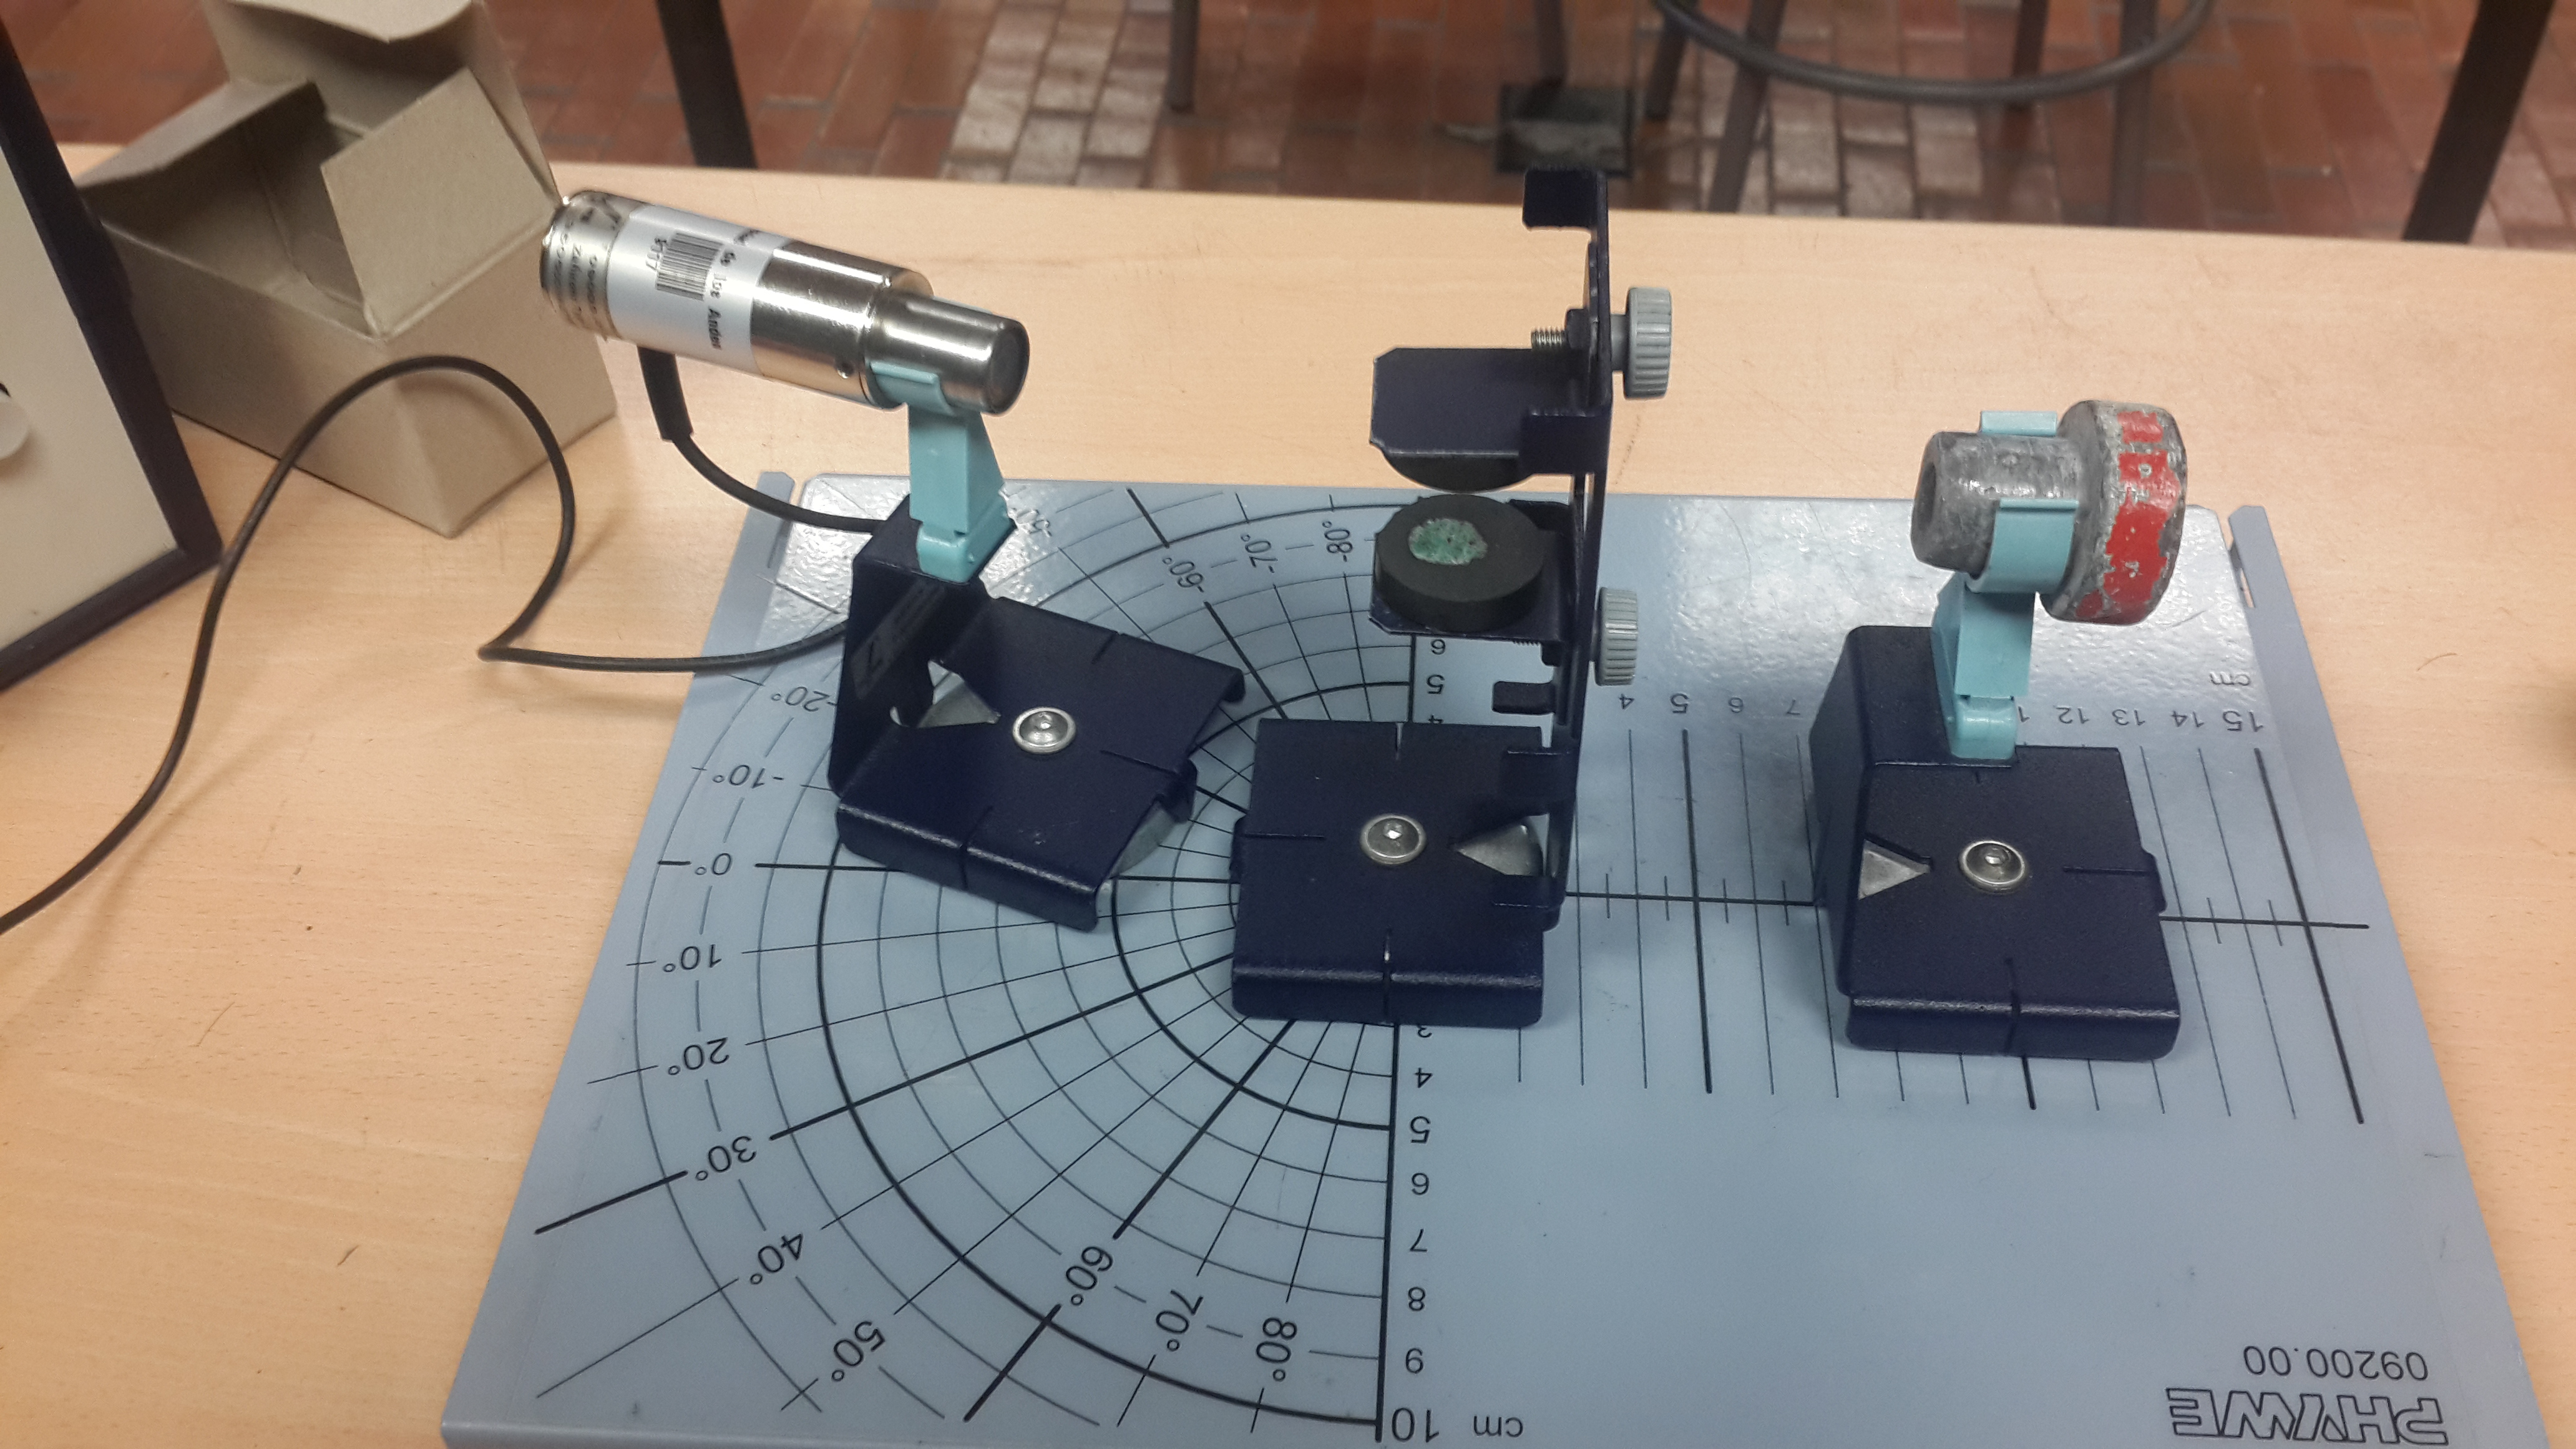
\includegraphics[width=0.5\textwidth]{radio1}
	\caption{ Montaje experimental usado para las mediciones con radio. }
	\label{fig: radio1}
\end{figure}

Los datos obtenidos se muestran en la tabla \ref{tabla7}. 

\begin{table}[h!]
	\caption{\label{tabla7}Conteos para el radio a diversas distancias.}
	\begin{ruledtabular}
		\begin{tabular}{|M{1.cm}|M{1.cm}|M{1.cm}|M{1.cm}|M{1.cm}|M{1.cm}|M{1.cm}|}
			Sep. (cm)   & $C_{1}$/\ \ \ \ \ \ \ \ \ 10 s & $C_{2}$/\ \ \ \ \ \ \ \ \ 10 s & $C_{3}$/\ \ \ \ \ \ \ \ \ 10 s & $C_{4}$/\ \ \ \ \ \ \ \ \ 10 s & $C_{5}$/\ \ \ \ \ \ \ \ \ 10 s & $\bar{C}$/\ \ \ \ \ \ \ \ \ 10 s\\
			\hline
			13 & 2323 & 2324 & 2331 & 2405 & 2314 & 2339.4\\\hline
			12 & 2805 & 2728 & 2736 & 2812 & 2776 & 2771.4\\\hline
			11 & 3199 & 3154 & 3122 & 3170 & 3267 & 3182.4\\\hline
			10 & 3697 & 3643 & 3665 & 3611 & 3598 & 3642.8\\\hline
			9  & 4354 & 4222 & 4410 & 4222 & 4398 & 4321.2\\\hline
			8  & 5134 & 5290 & 5177 & 5133 & 5133 & 5173.4\\\hline
			7  & 6330 & 6249 & 6113 & 6212 & 6246 & 6230\\\hline
			6  & 7452 & 7243 & 7295 & 7241 & 7260 & 7298.2\\\hline
			5  & 9375 & 9251 & 9360 & 9075 & 9284 & 9269 \\
		\end{tabular}
	\end{ruledtabular}
\end{table}

Cabe aclarar que se usó un tiepo de conteo de 10 s puesto que la muestra de radio proporcionadad era de 10 mg y se observó que si se dejaba durante 60 s se saturaba el dispositivo.\\

Los anteriores datos peromiten ver, como se esperaba, el radio es una sustancia extremadamente radioactiva y por tanto se tomaron todas las precauciones indicadadas para la manipulación de la misma.\\

Además de lo anterior, la figura \ref{fig: radio2} muestra la dependencia funcional de los datos de la tabla \ref{tabla7}. En dicha gráfica se evidenciando un aparente comportamiento exponencial  y decreciente de los datos. Allende de esto, es importante resaltar que aún con el tiempo corto de medición, el conteo aumentaba considerablemente al acercar la muestra al contador, indicando la gran magnitud de la radiación emitida por esta muestra.

\begin{figure}[h!]
	\centering
	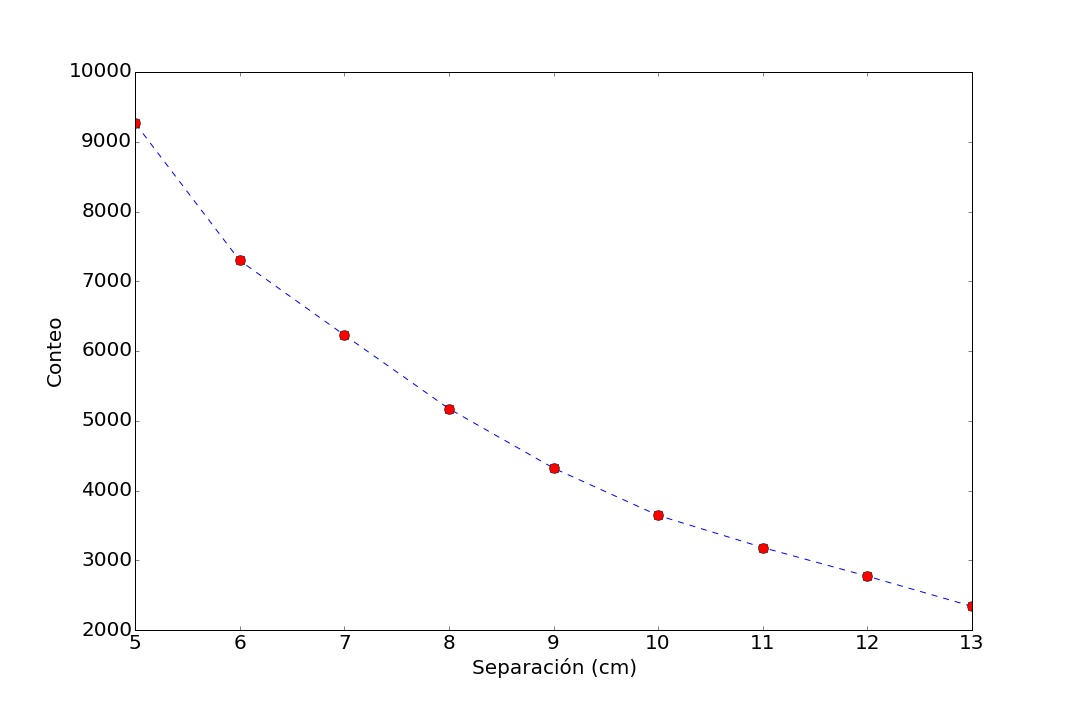
\includegraphics[width=0.5\textwidth]{radio2}
	\caption{Conteo en función de la distancia entre el radio y el contador.}
	\label{fig: radio2}
\end{figure}

\subsection{Rango de la raciación alfa}

El objetivo de este experimento es evidenciar y determinar cuantitativmente el bloqueo de la radiación alfa por una hoja de papel. El montaje experimental usado fue el mismo del experimento anterior, tan solo que entre el radio y el contador se antepuso una hoja de papel. Los resultados obtenidos se muestran en la tabla \ref{tabla8}

\begin{table}[h!]
	\caption{\label{tabla8}Conteos para el radio a diversas distancias con y sin papel.}
	\begin{ruledtabular}
		\begin{tabular}{|M{1.7cm}|M{1.7cm}|M{1.7cm}|M{1.7cm}|}
			Sep. (cm)    & $C_{aire}$ / 10 s & $C_{pap}$ / 10 s & \% alfa\\
			\hline
			5    & 9441 & 6414 & 32.06\\\hline
			6.5  & 6692 & 4576 & 31.61\\\hline
			8    & 4963 & 3413 & 31.23\\\hline
			9.5  & 4125 & 2629 & 36.26\\\hline
			11   & 3234 & 2217 & 31.44\\\hline
			12.5 & 2620 & 1753 & 33.09\\
		\end{tabular}
	\end{ruledtabular}
\end{table}

En promedio se obtuvo que el $32.61\%$ de la radiación proveniente de la muestra de radio era radiación alfa. Dado a que no se trabajó la muestra de radio sugerida en la guía \cite{guia} podemos observar un comportamiento prácticamente constante de la radiación bloqueada por la hoja de papel. Era imposible acercarse más dado a una inminente saturación del contador de Geiger. Dado esto, lo único que podemos concluir aquí es nuevamente la gran intensidad del radio frente a las demás fuentes radiactivas, puesto que inclusive su composición de radiación alfa es tres veces más grande que las de las muestras previamente examinadas.

\subsection{Materiales que bloquean la radiación beta}

Para diferentes materiales y diferentes grosores, se midió el comportamiento de la radiación que atraviesa los mismos. El objetivo es verificar que la radiación que atraviesa el material disminuye a medida que aumenta el grosor de dicho material. También se desea observar qué materiales bloquean mejor la radiación, particularmente la radiación beta. \\

De acueredo a lo mencionado en la guía\cite{guia} y los experimentos previos, sabemos que el plomo es el material que mejor dispersa este tipo de radiación pero desafortunadamente ,en el laboratorio no había suficientes capas de distintos grosores de estos materiales para desarrollar tomas de datos más completas. Teniendo en cuenta lo anterior, los datos obtenidos se muestran en la tabla \ref{tabla9}.

\begin{table}[h!]
	\caption{\label{tabla9}Conteos para el radio y diversos materiales de bloqueo.}
	\begin{ruledtabular}
		\begin{tabular}{|M{1.4cm}|M{1.4cm}|M{1.4cm}|M{1.4cm}|M{1.4cm}|}
			Mater./ Ancho (in)    & $C_{1}$ / 10 s & $C_{2}$ / 10 s & $C_{3}$ / 10 s & $\bar{C}$ / 10 s\\
			\hline
			Aluminio &  &  &  &\\\hline
			0 & 5802 & 5817 & 5738 & 5785.66\\
			0.02 & 790 & 777 & 764 & 777\\
			0.032 & 500 & 480 & 466 & 482\\
			0.04  & 387 & 341 & 374 & 367.33\\
			0.05  & 245 & 274 & 280 & 266.33\\
			0.063 & 233 & 223 & 226 & 227.33\\\hline
			Plomo &  &  &  &\\\hline
			0 & 5752 & 5710 & 5614 & 5692\\
			0.064 & 82 & 80 & 76 & 238\\
			0.125 & 72 & 73 & 68 & 71\\
			0.25  & 68 & 64 & 56 & 62.66\\\hline
			Plástico &  &  &  &\\\hline
			0 & 5725 & 5783 & 5724 & 5744\\
			0.03 & 1613 & 1697 & 1596 & 1635.33\\
			0.04  & 1233 & 1305 & 1255 & 1264.33\\
		\end{tabular}
	\end{ruledtabular}
\end{table}

A partir de los datos anteriores es evidente que lo mencionado previamente acrca de la efectividad del plomo para bloquear la radiación alfa. Esto puesto que es el que presenta la variación más significativa de los datos con y sin bloqueo. Además, dichos datos permiten también concluir nuevamente que la mayor parte de la radiación emitida por la muestra, en este caso el radio, es radiación beta y que, como se esperaba, entre mayor sea el grosor de la pantalla de bloqueo, menor es la radiación que deja pasar la misma.\\

Ahora bien, las gráficas de los datos se muestran en la figuras \ref{fig: bloqueo1},\ref{fig: bloqueo2} y \ref{fig: bloqueo3}.\\

\begin{figure}[h!]
	\centering
	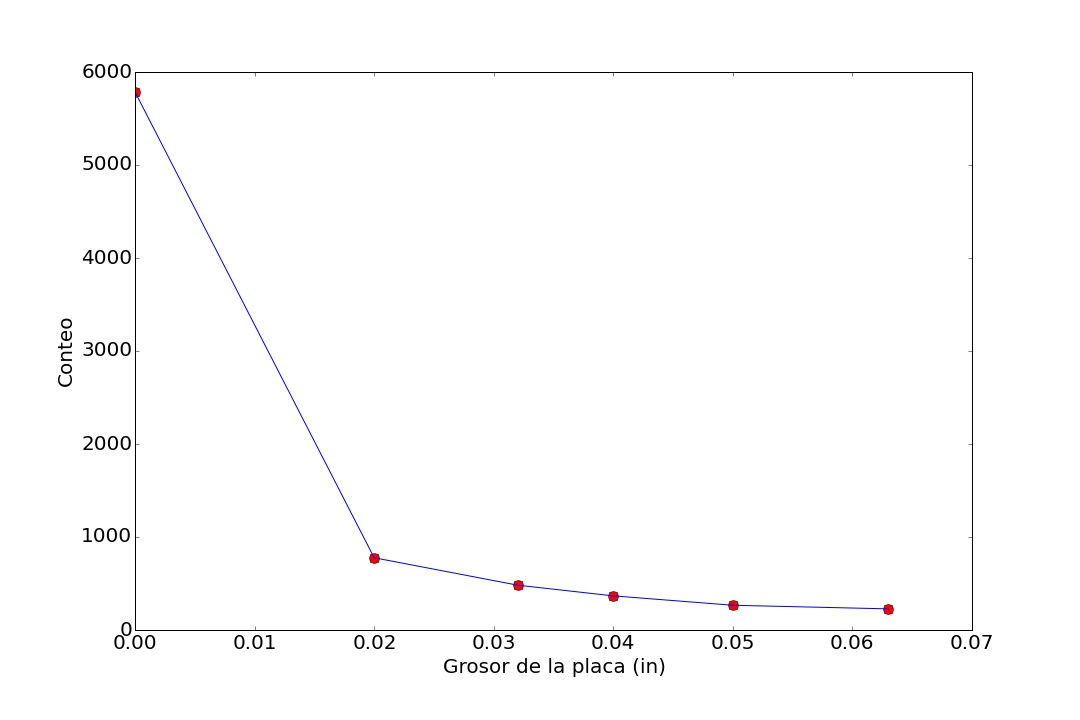
\includegraphics[width=0.5\textwidth]{bloqueo1}
	\caption{Conteo del radio para un bloqueo con aluminio.}
	\label{fig: bloqueo1}
\end{figure}


\begin{figure}[h!]
	\centering
	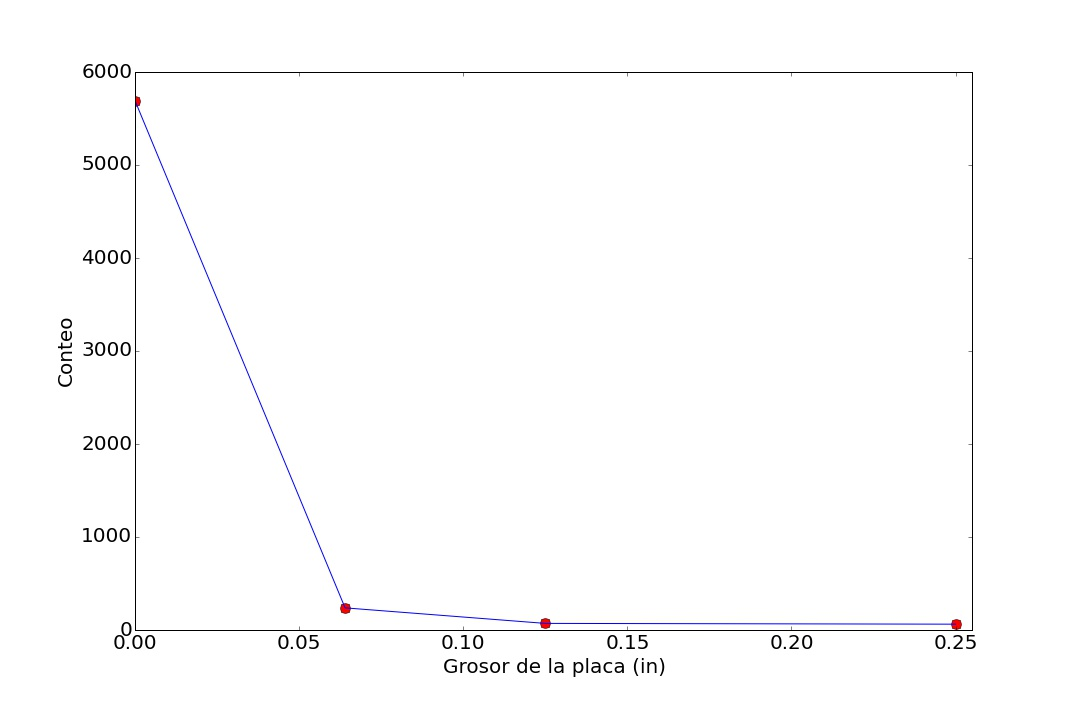
\includegraphics[width=0.5\textwidth]{bloqueo2}
	\caption{Conteo del radio para un bloqueo con plomo.}
	\label{fig: bloqueo2}
\end{figure}

\begin{figure}[h!]
	\centering
	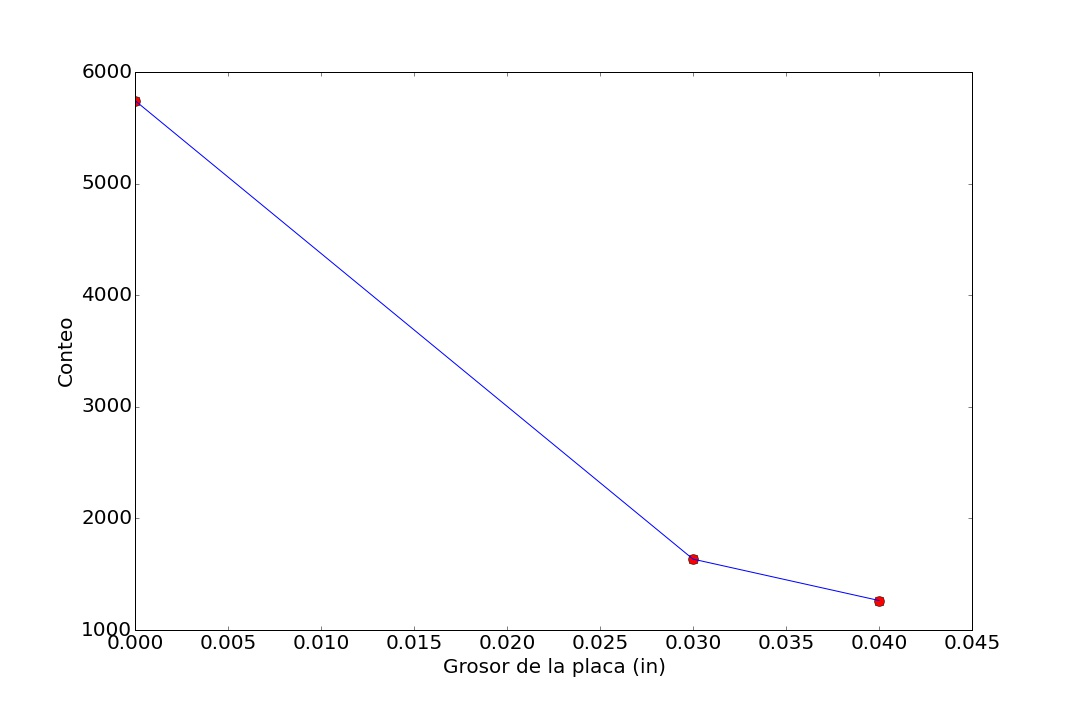
\includegraphics[width=0.5\textwidth]{bloqueo3}
	\caption{Conteo del radio para un bloqueo con plástico.}
	\label{fig: bloqueo3}
\end{figure}

Nuevamente, en las figuras anteriores se evidencia un decaimiento exponencial de la cantidad de radiación que penetra la placa a medida que aumenta el grosor de la misma. Este comportamiento se ajusta, con buena aproximación, a la ley exponencial dada por la ecuación \eqref{exponential}.

\begin{equation}
\label{exponential}
I = I_{0}e^{-\mu x}
\end{equation}

Donde $\mu$ es el coeficiente de reducción del material usado y $x$ es el grosor del material. Dado que no tenemos un conocimiento suficiente acerca de la ecuación presentada anteriormente, es intrascendente hacer una análisis matemático profundo de la misma, pero podemos concluir que dicha ecuación se ajusta apropiadamente a los datos obtenidos, y las gráficas anteriores evidencian, además del decrecimiento exponencial  mencionado anteriormente, la importancia del grosor de las barreras que bloquean la radiación, particularmente la radiación beta.

\subsection{Radiación beta y campos magnéticos}

En este experimento se pretendía observar el comportamiento del conteo de radiación al interponer verticalmente un campo magnético entre la fuente radioactiva y el contador. Además, se variaron los ángulos entre la muestra y el contador para observar la dirección de desvío de la radiación. La idea es que el contador Geiger barra todos los ángulos tal y como se muestra en la figura \ref{fig: montaje2}, haciendo un mapeo de las trayectorias \footnote{Como estamos considerando partículas cuánticas no podemos hablar de trayectorias definidas, sin embargo analizaremos en que zonas es más probable encontrar partículas $\beta$ dispersadas por la acción del campo.} de las partículas. Luego de hacer lo mencionado previamente, se cambió la disposición de los imanes con el fin de invertir el campo magnético, y se realizó nuevamente la toma de datos.\\

\begin{figure}[h!]
	\centering
	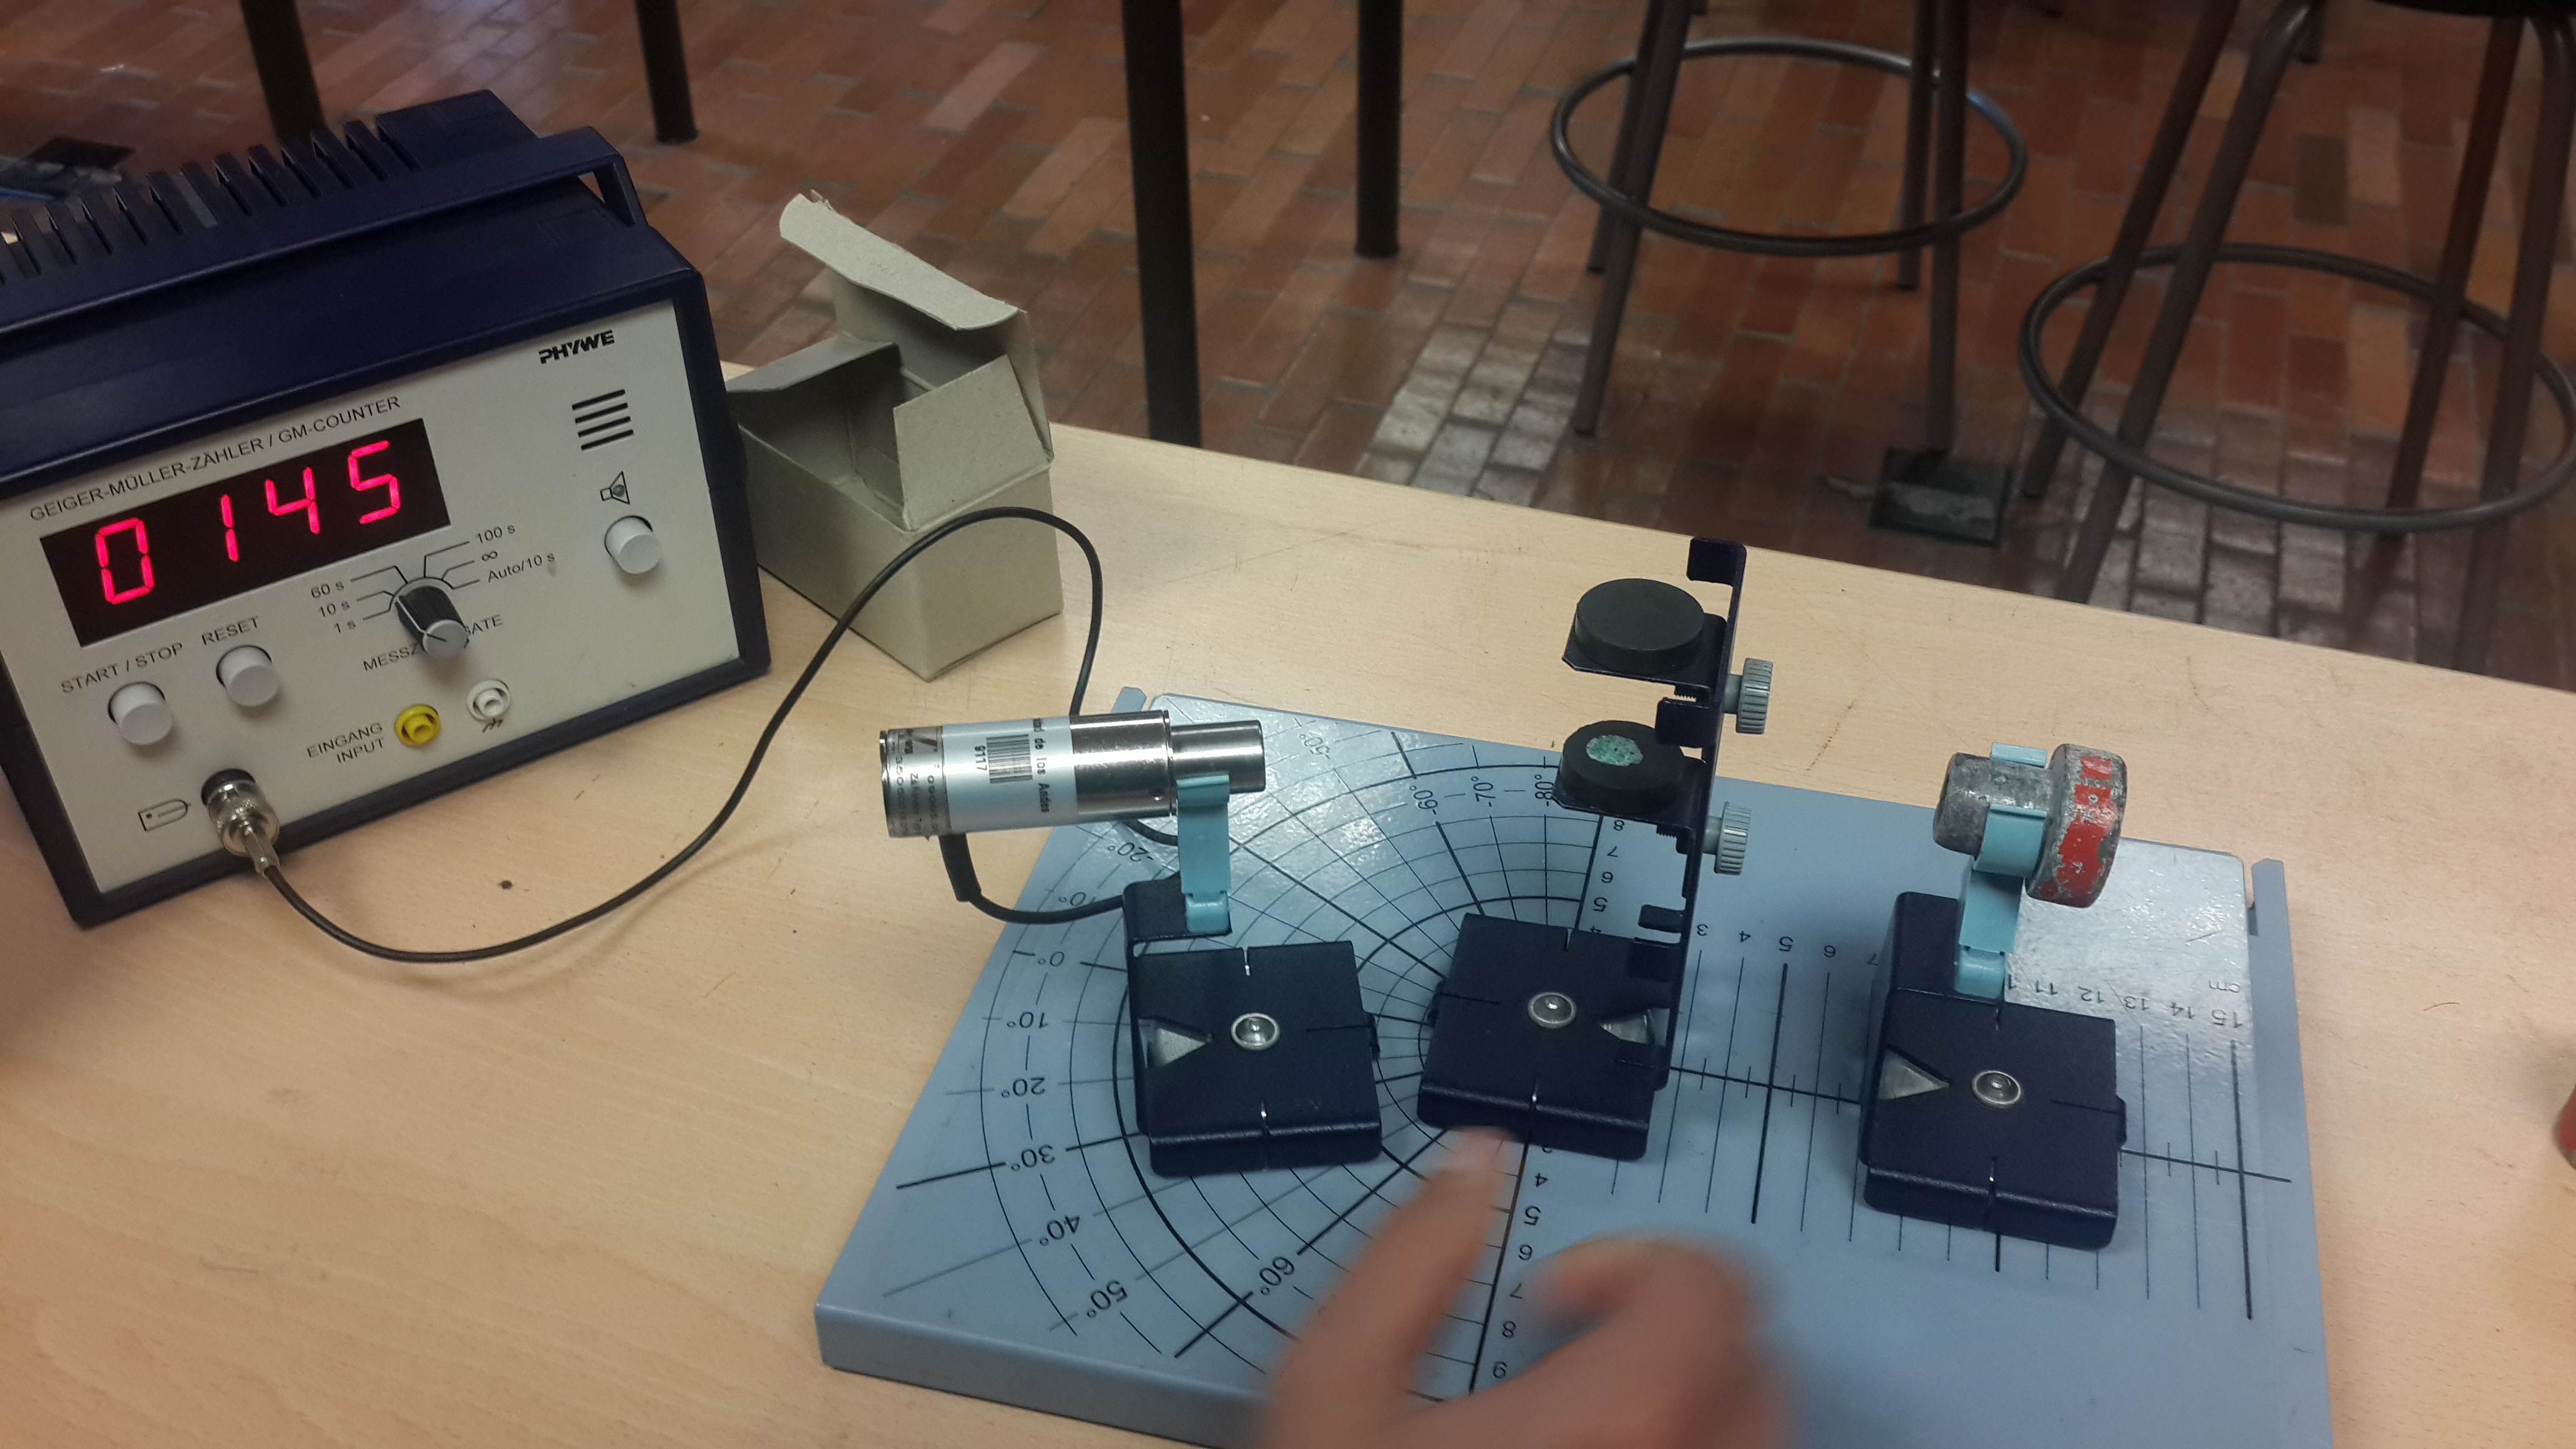
\includegraphics[width=0.5\textwidth]{montaje2}
	\caption{Conteo con un campo magnético entre el radio y el contador.}
	\label{fig: montaje2}
\end{figure}

Los datos obtenidos se muestran en la tabla \ref{tabla10} y la gráfica de los mismos se muestra en la figura \ref{fig: angles}.\\

\begin{table}[h!]
	\caption{\label{tabla10}Conteos al interponer un campo magnético entre el radio y el contador.}
	\begin{ruledtabular}
		\begin{tabular}{|M{2.7cm}|M{2.7cm}|M{2.7cm}|}
			Ángulo (sexagesimal) & Imanes / 10 s & Imanes invertidos / 10 s \\
			\hline
			0  & 877 & 1383 \\\hline
			10 & 843 & 1183 \\\hline
			20 & 870 & 1000 \\\hline
			30 & 774 & 707 \\\hline
			40 & 565 & 515 \\\hline
			50 & 437 & 381 \\\hline
			60 & 485 & 361 \\\hline
			70 & 540 & 497 \\\hline
			80 & 516 & 459 \\\hline
			90 & 457 & 413 \\\hline
			-10 & 1034 & 1825 \\\hline
			-20 & 1266 & 1749 \\\hline
			-30 & 1846 & 1608 \\\hline
			-40 & 1884 & 1162 \\\hline
			-50 & 1618 & 767 \\\hline
			-60 & 1275 & 711 \\\hline
			-70 & 1144 & 723 \\\hline
			-80 & 1002 & 635 \\\hline
			-90 & 875 & 648 \\\hline
		\end{tabular}
	\end{ruledtabular}
\end{table}

\begin{figure}[h!]
	\centering
	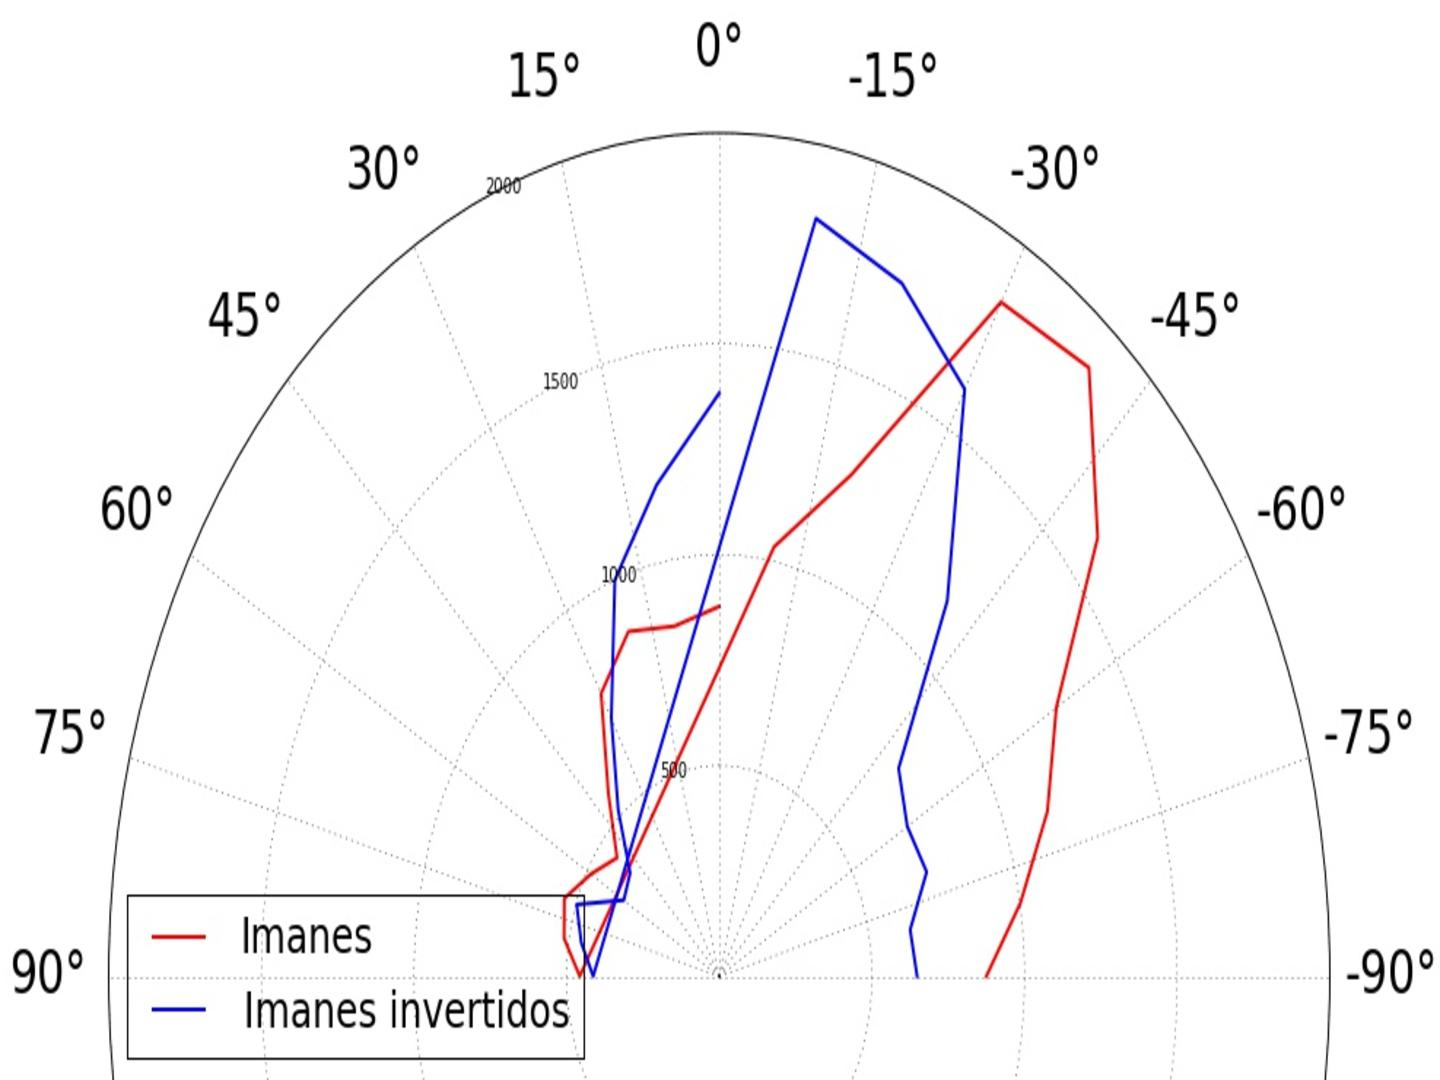
\includegraphics[width=0.5\textwidth,height=0.2\textheight]{angles}
	\caption{Conteo con un campo magnético entre el radio y el contador.}
	\label{fig: angles}
\end{figure}

En la susodicha figura \ref{fig: angles} se puede observar que la radiación presenta máximos relativamente alejados de la posición $0^o$, los cual es un clara consecuencia de la presencia del campo magnético, puesto que su acción consiste precisamente en derviar un cierto ángulo las partículas radiadas. No obstante, es inusual que los máximos en ambos casos se presenten hacia el mismo "lado", esto porque al cambiar la disposición de los imanes se está invirtiendo el campo magnético y por ende se está modificando la dirección en la cual las partículas son desviadas en otra dirección. Dicho comportamiento anómalo puede ser explicado nuevamente por el hecho de que otros grupos también estuvieran trabajando con radio en el momento de tomar las medidas.\\

Allende de lo anterior, es preciso mencionar que cuando se interpone un campo magnético entre el contador y la muestra, el máximo del conteo de radiacón en función del ángulo se mueve de la posición $0^o$ (su posición natural) debido a que el campo magnético desvía las partículas radiadas. Sin embargo algunas partículas altamente energéticas no se ven afectadas por el campo y generan nuevamente un pico en la posición natural. Si se aumenta la intensidad del campo magnético, el pico a cero grados desaparece puesto que son pocas las partículas que logran atravesar el campo interpuesto.



\subsection{Radiación gamma en un campo magnético}

El objetivo de este experimento es determinar si la radiación gama se ve afectada o no por campos magnéticos. El montaje propuesto consiste en interponer entre el radio y el contador una placa de plomo lo suficientemente gruesa de tal forma que solo pase la radiación gamma y tomar datos de conteos con y sin imanes entre la muestra y el contador.\\

Los datos obtenidos se muestran en la tabla \ref{tabla11}.

\begin{table}[h!]
	\caption{\label{tabla11}Conteos de radiación gamma.}
	\begin{ruledtabular}
		\begin{tabular}{|M{2.7cm}|M{2.7cm}|M{2.7cm}|}
			Medición $\#$ & Imán-Plomo / 10 s & Plomo / 10 s\\
			\hline
			1 & 77 & 85 \\\hline
			2 & 98 & 78 \\\hline
			3 & 76 & 99 \\\hline
			4 & 81 & 101 \\\hline
			5 & 79 & 83 \\\hline
			Promedio & 81.8 & 89.2\\
		\end{tabular}
	\end{ruledtabular}
\end{table}

El error de los datos de la columa "Plomo" fue de $s = 9.36$ conteos / 10 s, y al comparar con el promedio de la columna "Imán-Plomo" vemos que el valor $81.9$ está dentro del error $s$ calculado. Dado lo anterior podemos concluir que las partículas que componen la radiación gamma no poseen carga eléctrica puesto que no se ven afectadas por campos magnicos perpendiculares a su trayectoria, además de verificar nuevamente que el plomo bloquea completamente la radiación beta.\\

\subsection{Variación de la intensidad de radiación con el tiempo}

La idea de este experimento es confinar algunas partículas emitidas por una fuente radioactiva en un recipiente para examinar su decaimiento en el tiempo.

Los datos obtenidos se mustran en la tabla \ref{tabla12}.

\begin{table}[h!]
	\caption{\label{tabla12}Conteos de radiación gamma.}
	\begin{ruledtabular}
		\begin{tabular}{|M{2.7cm}|M{2.7cm}|}
			Segundos & Conteo\\
			\hline
			60  & 44 \\\hline
			120 & 39 \\\hline
			180 & 38 \\\hline
			240 & 29 \\\hline
		\end{tabular}
	\end{ruledtabular}
\end{table}

Se puede observar de forma clara que la intensidad de la radiación disminuye con el tiempo. No obstante, es importante resaltar que las medidas no son totalmente confiables puesto que no difieren mucho del conteo usual del aire. Esto puede ser explicado por múltiples fuentes de error en este experimento, entre ellas el hecho de que el contador no se ajustara perfectamente al recipiente proporcionado y el hecho de que posiblemente el inyector que se tomó tuviera deteriorada la manta radioactiva en su interior. 

\subsection{Back-scattering de la radiación beta}

La radiación "reflejada" por un cierto material, puede ser utilizada para identificar diversos tipos de materiales. Precisamente el objetivo de este experimento es caracterizar dicha reflección con los materiales disponibles en el laboratorio.\\

El montaje experimental consiste en ubicar el radio y el contador en un ángulo de $60^o$ entre sí, y tomar datos sobre los conteos registrados. Los datos obtenidos se muestran en la tabla \ref{tabla13}.

\begin{table}[h!]
	\caption{\label{tabla13}Conteos de back-scattering de la radiación beta.}
	\begin{ruledtabular}
		\begin{tabular}{|M{1.5cm}|M{1.5cm}|M{1.5cm}|M{1.5cm}|M{1.5cm}|}
			Material & $C_{1}$ / 10 s & $C_{2}$ / 10 s & $C_{3}$ / 10 s & $\bar{C}$ / 10 s\\
			\hline
			Aire & 382 & 411 & 407 & 400\\\hline
			Plomo & 783 & 729 & 805 & 772.33\\\hline
			Aluminio & 480 & 479 & 531 & 496.66\\\hline
			Metal no id. & 526 & 522 & 543 & 530.33\\
		\end{tabular}
	\end{ruledtabular}
\end{table}
 
Nuevamente, la mayor intensidad fue registrada para el plomo dado que este material es muy efectivo para bloquear la radiación beta. Es importante mencionar que las mediciones eran muy sensibles ante pequeñas variaciones en las distancias tanto de la muestra como del contador, por tanto se tuvieron que repetir algunas mediciones que eran inconsistentes con respecto a los demás datos. Además,dada la cercanía entre los últimos dos datos se puede concluir que potencialmente el metal no identificado era aluminio ligeramente más grueso que la muestra anterior.

\subsection{Usos alternos de la radiación beta}

Una característica notable sobre la radiación $\beta$ es que cambia  su intensidad de acuerdo a la cantidad de material que hay en un recipiente que bloquea la radiación. De esta manera se puede determinar qué tan lleno está un recipiente que no se puede observar. Usando el montaje mostrado en la figura \ref{fig: lleno}, se trató de determinar qué tan lleno estaba un tubo proporcionado en el laboratorio.\\

\begin{figure}[h!]
	\centering
	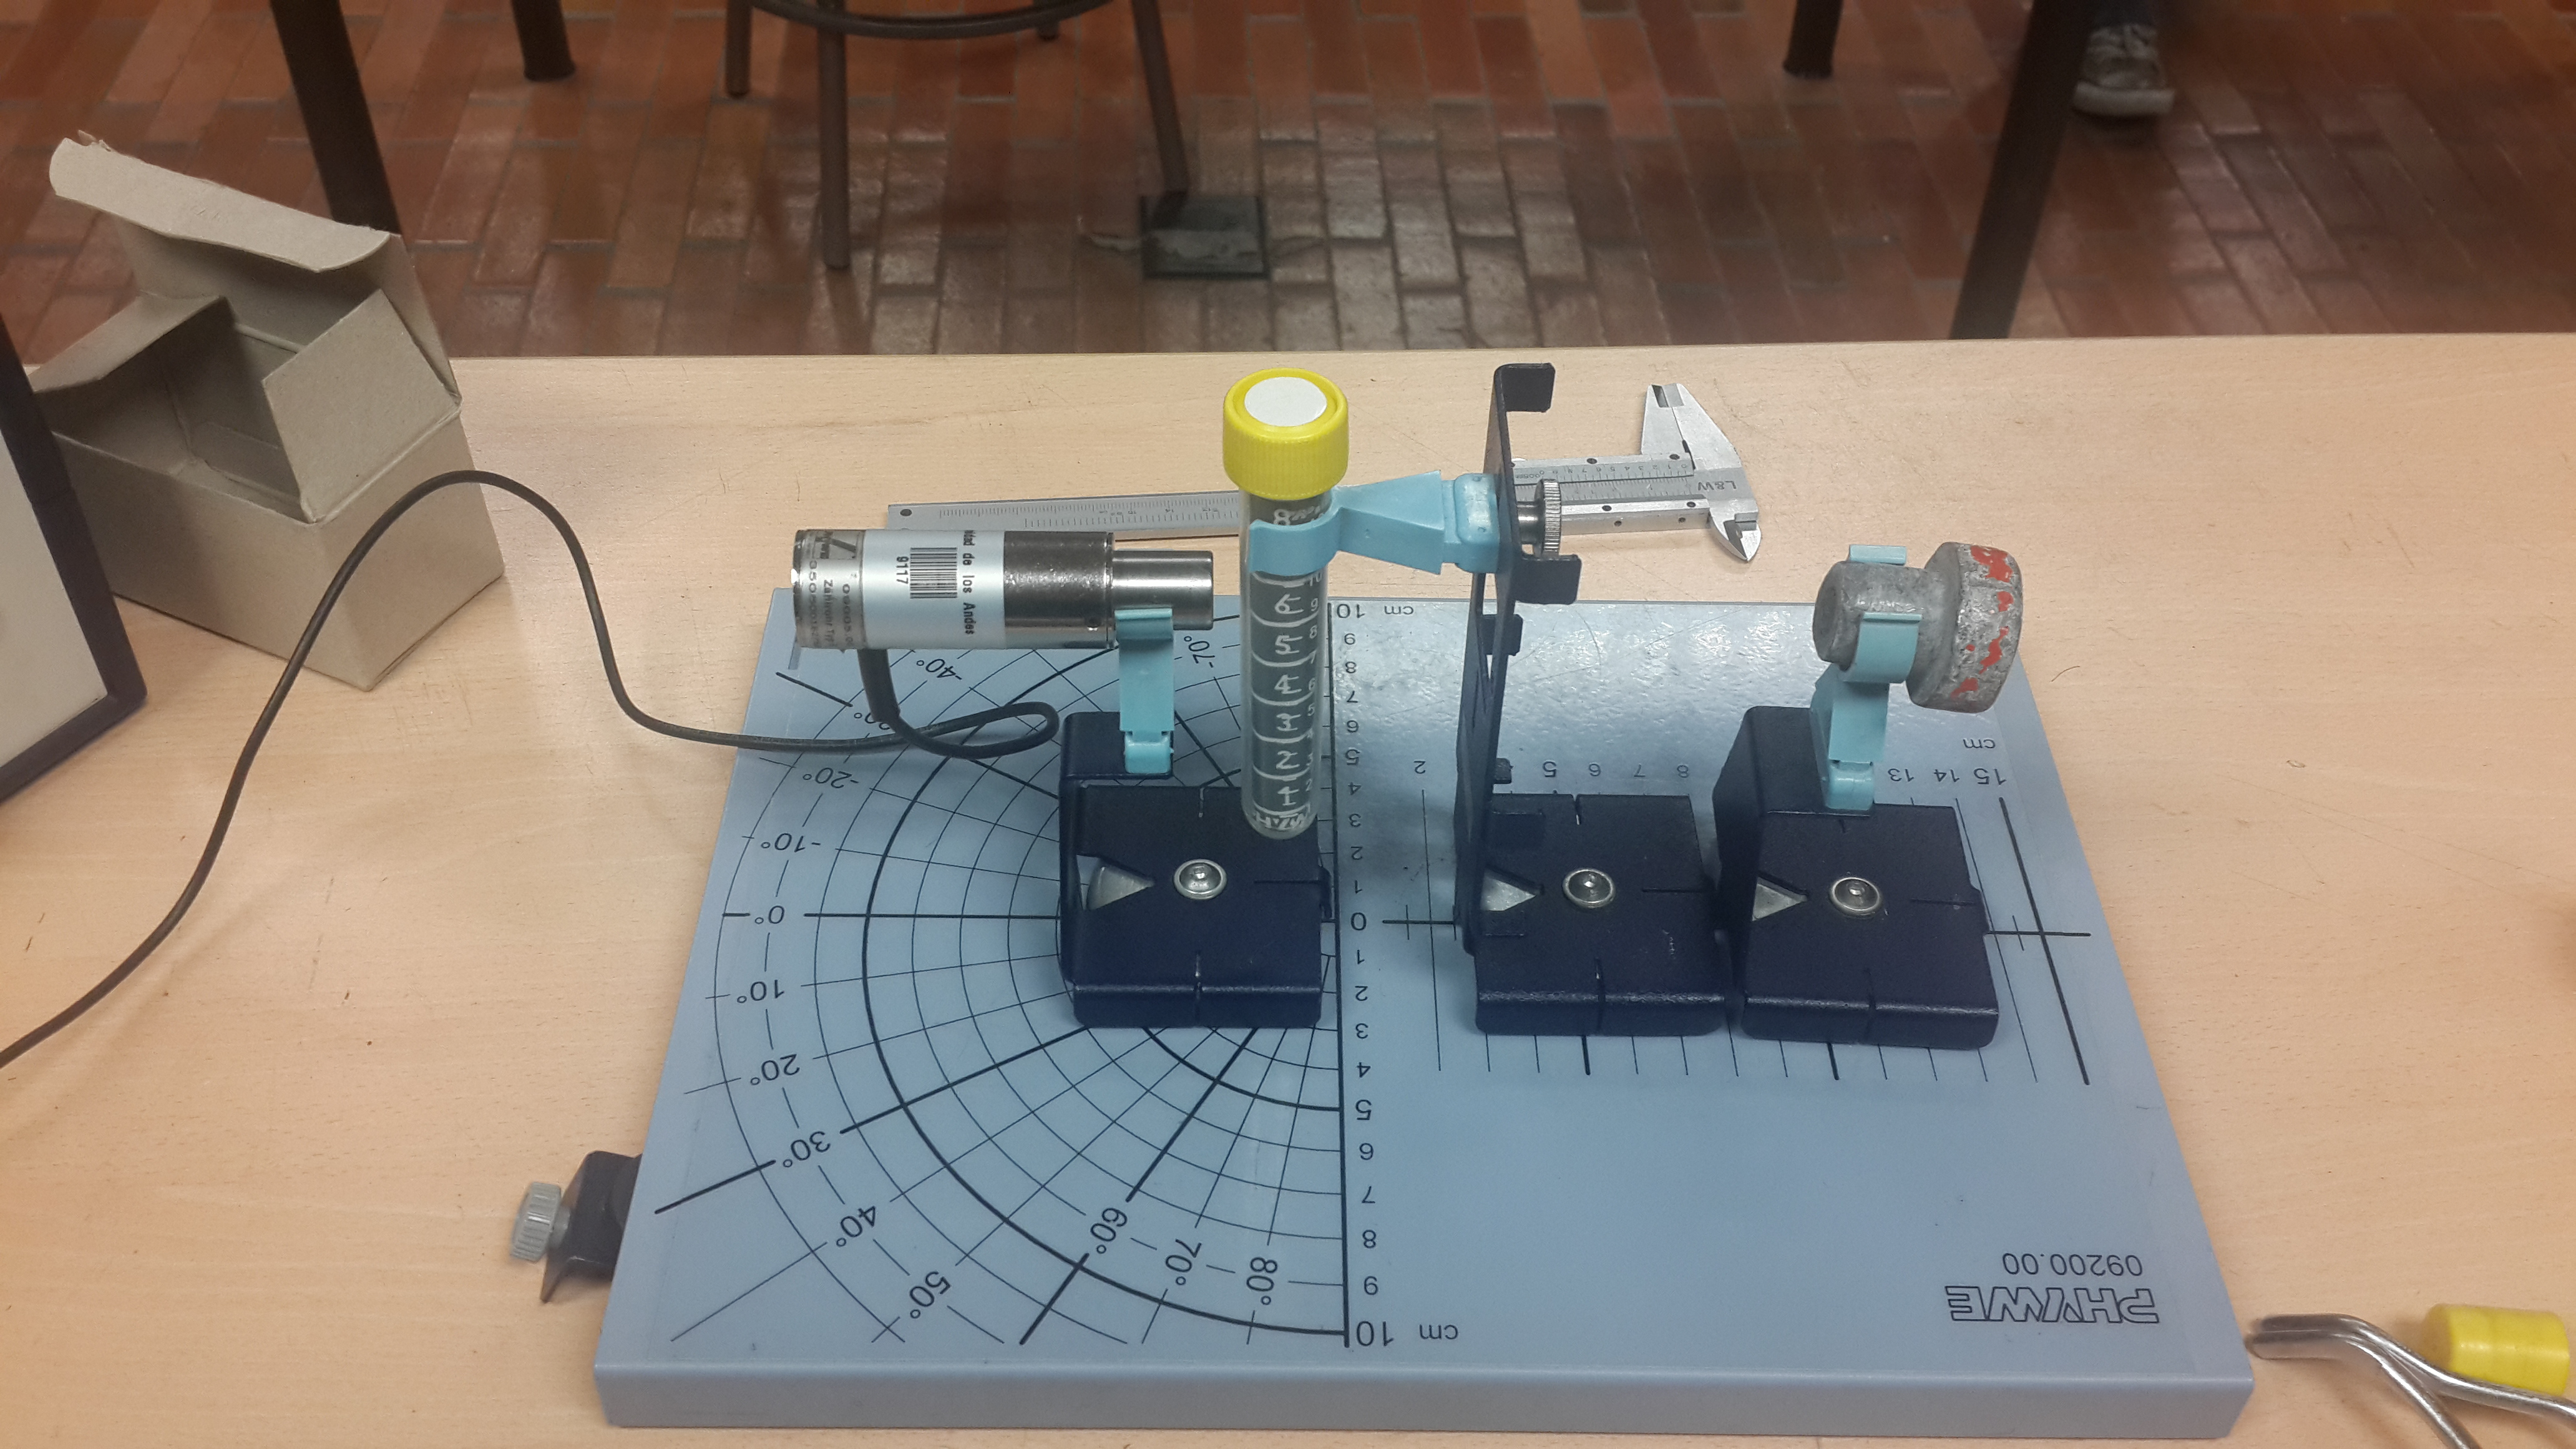
\includegraphics[width=0.5\textwidth]{lleno}
	\caption{Conteo para determinar qué tan lleno está un recipiente sin necesidad de abrirlo.}
	\label{fig: lleno}
\end{figure}

Los datos obtenidos se muestran en la tabla \ref{tabla14}.

\begin{table}[h!]
	\caption{\label{tabla14}Conteos usando un recipiente como bloqueo.}
	\begin{ruledtabular}
		\begin{tabular}{|M{4.5cm}|M{4.5cm}|}
			Altura (cm) & $C$ / 10 s \\
			\hline
			1 & 1860 \\\hline
			2 & 1776 \\\hline
			3 & 1880 \\\hline
			4 & 1934 \\\hline
			5 & 1849 \\\hline
			6 & 1872 \\\hline
			7 & 1881 \\
		\end{tabular}
	\end{ruledtabular}
\end{table}

Dado que todas las medidas son muy cerrcanas entre sí podemos concluir que el tubo proporcionado esta vacío, y esto se comprobó puesto que al teminar las medidiciones de destapó dicho recipiente y se verfició que no contenía nada en su interior. Por faltta de tiempo no se tomaron medidas con otros recipientes.

\subsection{Radiación beta y hojas de papel}

El montaje experimental utilizado en este último experimento es análogo al mostrado a la figura \ref{fig: angles} tan solo que esta vez se hacía incidir la radiación sobre múltiples capas de papel.\\

La última aplicación posible del uso de radiación para la caracterización de materiales es que se puede detectar su grosor. Se realizó una calibración con la radiación detectada para distintos grosores de papel logrados al sobreponer múltiples hojas de papel una sobre la otra. Los datos obtenidos se muestran en la tabla \ref{tabla15}.\\

\begin{table}[h!]
	\caption{\label{tabla15}Conteos de la radiación beta incidiendo sobre mpultiples hojas de papel.}
	\begin{ruledtabular}
		\begin{tabular}{|M{1.5cm}|M{1.5cm}|M{1.5cm}|M{1.5cm}|M{1.5cm}|}
			$\#$ de hojas & $C_{1}$ / 60 s & $C_{2}$ / 60 s & $C_{3}$ / 60 s & $\bar{C}$ / 60 s\\
			\hline
			1 & 2569 & 2599 & 2541 & 2569.66\\\hline
			2 & 2666 & 2607 & 2637 & 2636.66\\\hline
			3 & 2680 & 2710 & 2735 & 2708.33\\\hline
			5 & 2712 & 2788 & 2681 & 2727\\\hline
			8 & 2693 & 2777 & 2658 & 2709.33\\\hline
		\end{tabular}
	\end{ruledtabular}
\end{table}

Dado a que no hay variaciones significativas a medida que se aumenta el número de hojas, podemos decir que el grosor de las mismas no es lo suficiente para que las mediciones sean confiables. Además, el papel utilizado no era completamente blanco, por lo cual el constituyente de la tinta con la que fue impreso dicho papel pude haber afectado fuertemente las mediciones realizadas.

\section{\label{conclusiones}Conclusiones}

\begin{itemize}
	\item La radiación es un fenómeno natual que los seres vimos toleramos constantemente en la vida cotidiana.
	
	\item Múltiples materiales pueden bloquear diversos tipos de radiación, entre ellos el papel, el aluminio y el plomo. No obstante, el papel solo bloquea la radiación alfa, el plomo bloquea la radiación alfa y beta, y ninguno de los materiales proporcionados en el laboratorio pudo bloquear la radiación gamma.
	
	\item El radio es una fuente radioactiva de ata intensidad y se deben tomar todas las precacuciones necesarias a la hora de manipularlo, tales como no tocarlo directamente con las manos y sacarlo de cun contenedor única y exclusivamente el tiempo necesario para tomar datos.
	
	\item Minerales radioactivos como la columbita pueden producir diversos tipos de radiación de baja intensidad. Y no solo la columbita sino también la manta incandescente y el radio, emitían los tres tipos de radiación más conocidos, a saber, radiación alfa, beta y gamma.
	
	\item El back scattering de radiación por un material determinado puede ser utilizado para la caracterización de un material determinado.
	
	\item El campo magnético afecta la trayectoria de las ciertas partículas emitidas por fuentes radioactivas. En particular, en el experimento \textit{Radiación gamma en un campo magnético} pudimos verificar que las partículas que constituyen la radiación gamma no poseen carga eléctrica. Esto permite verificar, a su vez, la caracterización de este tipo de radiación hecha en la sección  \textbf{INTRODUCCIÓN} 
	
	\item Si bien, el scattering de partículas radioactivas permite determinar el grosor de materiales, las mediciones realizadas en el experimento no arrojaron resultados significativos con respecto al número de hojas de papel utilizadas .
\end{itemize}

\begin{thebibliography}{99}
\
\\
\bibitem{guia} Guía \textit{Radioactividad} proporcionada para el desarrollo del laboratorio.\\
\bibitem{hyperphyisics} Informacion consultada en http://hyperphysics.phy-astr.gsu.edu/hbase/nuclear/radact.html.\\
\bibitem{wikipedia} Información consultada en https://en.wikipedia.org/wiki/Radioactive\_decay.\\
\bibitem{error} Taylor, J.R., \textit{An Introduction to Error Analysis}. University Science Books, Sausalito, California. 2nd edition, 1982.\\
\end{thebibliography}

\end{document}
%
% ****** End of file apssamp.tex ******
